%%%%%%%%%%%%%%%%%%%%%%%%%%%%%%%%%%%%%%%%%%%%%%%%%%%%%%%%%%%%%%%%%%% 
%                                                                 %
%                            CHAPTER Four                         %
%                                                                 %
%%%%%%%%%%%%%%%%%%%%%%%%%%%%%%%%%%%%%%%%%%%%%%%%%%%%%%%%%%%%%%%%%%% 

\chapter{USE CASES}
In this chapter, two use cases are implemented based on semantic importance and the sequential stream reasoning architecture.
The use cases leverage different combinations of semantic importance aspects which support different window management strategies.
This chapter aims to show how semantic importance is determined, deployed in stream reasoning use cases, as well as how semantic importance impacts the system performance. 
%
\section{Soccer Offside Detection}
This use case detects soccer offside offence with a particular focus on the accuracy, error and running performance of window management strategies based on the semantic importance.
%
\subsection{Background}
Soccer (a.k.a. association football) is one of the most influential and competitive sports across the globe. 
In soccer games, one common offence among others is called ``offside offence''. 
FIFA\footnote{https://www.fifa.com/ (Date Last Accessed: Mar. 20, 2018)} defines it in a comprehensive way.
For details, please refer to Rule 11 in FIFA laws of the game \cite{federation2016laws}.
However, it is worth to mention a key point: that a player is at an offside position is determined at the moment when the ball is played by this player's teammate; once identified, this status will be retained until the ball is touched again. 
For example, when Player A2 passes the ball to his teammate Player A1 who is at an offside position, even if Player A1 relocates himself to touch the ball in an onside position, it is still considered as an offside offence. 

In order to give accurate offside decisions, a linesman (assistant referee) in his/her assigned half field needs to keep close track of the second-last defender, the ball-passing moment and any attackers at the offside position.
However, the fast tempo and heated atmosphere of the soccer game, together with linesmen' limited visual field and potential tiredness, can contribute to erroneous offside judgments, which may allow illegal attacking opportunities or disallow legal ones, and consequently affect the outcome of the game.

A number of studies have focused on the prevalence of offside mistakes by linesmen. 
\cite{catteeuw2010offside} investigates the accuracy of offside judgments in the English Premier League, with a reported error rate of 17.5\%. This is possibly because the English linesmen tend not to signal in doubtful situations, so there is an overall bias towards non-flag errors (773 non-flag errors vs 95 flag errors).
Another study \cite{helsen2006errors} analyzes 337 offside judgments in all 64 games during the 2002 FIFA World Cup, and finds the error percentage to be 26.2\%.
\cite{catteeuw2010offside} also examines the accuracy of offside judgments during the 2006 FIFA World Cup, and finds an error rate of 7.6\%, significantly lower than that of \cite{helsen2006errors}.
This study argues that the reduction in error rate might be due to different approaches the authors take to count errors.
The study also reveals higher rate of non-flag errors (9.6\%) than flag errors (6.9\%), within the overall error rate of 7.6\%.

A 2013 report \cite{fowler2010feasible} analyzes several offside detection systems, and proposes a number of evaluation criterion such as accuracy, fairness, system delays, feasibility, cost and intrusiveness of the system development and deployment.
Offside event detection methods may be based on various technologies, such as image processing \& computer vision \cite{naidoo2006soccer}, and stereo vision tracking  \cite{borg2007detecting}.
In addition to vision-based tools, sensor-enabled equipment is also employed in this scenario \cite{regan2013sports} \cite{garcia2011wireless}.
An example is the sports vest provided by GPsports\footnote{http://gpsports.com/ (Date Last Accessed: Mar. 20, 2018)}, which has been already used in the professional soccer.
The GPsports vest is equipped with sensors that track volume, intensity and work rate of matches played or training by recording and analyzing real-time data such as player position, velocity and heart rate.
According to its official website, this system has been successfully adopted by 150 clients of 10 sports, including prestigious soccer teams such as Real Madrid C.F. and Chelsea F.C.

Overall, sensor-based systems have great advantages by providing real-time, high-frequency, high-speed motion data of all available participants, but they lack the ability to determine the precise positions of players with reference to relevant boundaries required for offside calculations. 
Vision-based technologies are getting more precise for player boundary proximity detection, but output credibility and cost of computation have been major concerns.

The fact that gears like the GPsports vest have become more pervasive provides both opportunities and challenges for soccer. 
The opportunities lie in analysis of the real-time streaming data for players' kinetic and biological statistics such as location, velocity, acceleration, heart rate, breathing, and so forth. 
The challenges also come with the data: these systems require technologies to efficiently process constantly-updating, high volume and heterogeneous real-time streaming data in order to better analyze player performance for coaches, provide timely input of relevant officiating content for referees, and help spectators to enjoy the match. 
While contemporary stream processing systems are able to store and query low-level data at high speed, they do not typically have a framework to also furnish higher-level information that is implicit in the data.  
This is because this implicit information (e.g. player tiredness, opponent strategy, etc.) is not directly revealed by a stream processing system, which can only process explicit data (e.g. player position, velocity) and support window-based queries.  
In a soccer scenario, for example, a pure stream processing system would not be able to tell the coach that his left fullback is becoming tired and could be exploited by the opponent's fast right winger, or make other tactical suggestions. 
%
\subsection{Approach}
Timestamp metadata, such as arrival timestamp, has each been investigated as a key feature for window management.
But it only scratches the surface of possible ways to establish a specific window management strategy. 
Overall, a good window management strategy implementation will look for the right combination of heuristic guidelines that best capture the important information for the queries at hand.
In considering these heuristics, there are certain domain-independent contributors (e.g. time and use frequency), but there are also domain-dependent contributors that stem from the requirements of the particular use case, such as the goal of the use case, the specific answers expected from the data, the background knowledge and constraints, specific space and time limitations, etc. 
Knowing these requirements, humans can often determine efficient policies about which data will contribute to the query. 
For example, because we know that only an attacker can commit an offside offence, we can conclude that positional data for the defenders will never contribute to the query, and so is unimportant and can be flushed from the window.  
%
\subsection{Date Stream}
The data was collected during a practice game played on a half-sized soccer field. 
It includes information for one referee, two teams, eight players (including one goalkeeper) per team, and four balls (one ball is in play while the other three are backup balls). 
Sensors, installed in the center of the balls, and on the shin-guards and gloves of the players and referees, constantly stream kinetic data at high frequencies, such as position, velocity, acceleration, and directional vector. 
The ball sensor is 2000Hz, the player/referee sensor is 200Hz.
For more details, please refer to \cite{mutschler2013debs}.

The game duration is two halves of thirty minutes each.
In addition to the streaming data, a full video of the game is provided. 
This use case hires a soccer referee certified by United States Soccer Association and National Intercollegiate Soccer Officials Association as a domain expert.
He reviewed the game video and provided a list of suggested officiating decisions for a total of twenty relevant scenarios, where decisions are given as ``offside offence'', ``no offence'', or ``unsure''.
His decisions are used as a ground truth to evaluate system precision.
%
\subsection{Ontology}
For this use case, the overall ontologies are modularized into three sub-ontologies:
(1) the individual ontology that encodes the specific match information such as teams and players in each team;
(2) the offside offence ontology that concentrates on the offside offence detection from the streaming data;
(3) the query relevance ontology that focuses on filtering out offside-irrelevant data from the streaming data.

\begin{figure}[!htbp]
	\centering
	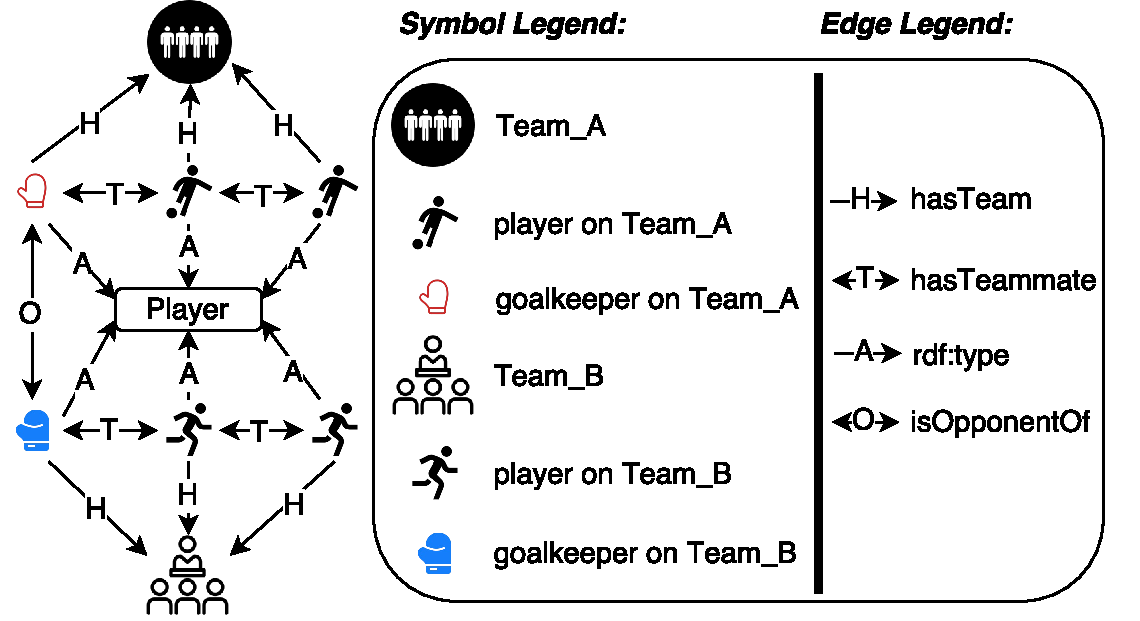
\includegraphics[width=5in]{img/5-matchOnto}
	\caption{\textbf{Individual Ontology}}
	\label{fig:matchOnto}
\end{figure}

For the purpose of illustration, three players are drawn from each team in Figure \ref{fig:matchOnto}.
All of the player individuals have a type of \textbf{Player}, which is a concept in the offside offence ontology.
\textit{hasTeam} is a functional property with a domain of \textbf{Player} and a range of \textbf{Team}.
Both \textit{hasTeammate} and \textit{isOpponentOf} are symmetric properties with \textbf{Player} as their domain and range.
\textit{hasTeammate} is transitive, meaning that a player can be his own teammate.\footnote{This is a modeling choice, not an error.}
\textit{isOpponentOf} is encoded only between two goalkeepers.

\begin{figure}[!htbp]
	\centering
	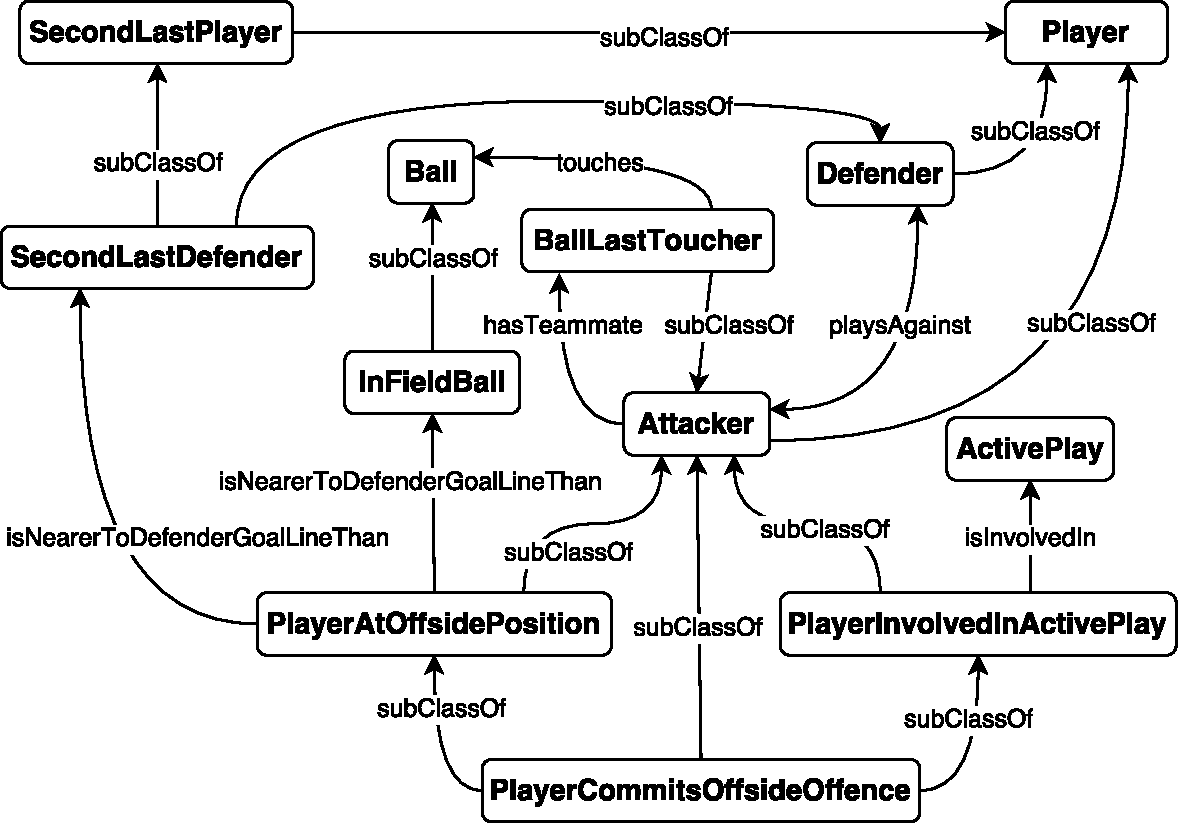
\includegraphics[width=5in]{img/5-soccerOnto}%
	\caption{\textbf{Offside Offence Background Domain Ontology}}
	\label{fig:soccerOnto}
\end{figure}

Figure \ref{fig:soccerOnto} shows the major classes and relations in order to describe the concept of the offside offence.
When developing this ontology, FIFA laws of the game \cite{federation2016laws} is used as the text corpus to extract a list of the offside relevant terms.
The term list was then carefully examined and curated to create a conceptual model, which was refined and extended to create the offside offence ontology\footnote{Please refer to https://tw.rpi.edu/web/Courses/Ontologies/2016/projects/soccer (Date Last Accessed: Mar. 20, 2018) for more details.}.
In a soccer game, usually the player who is touching the ball is considered to be an attacker, along with his teammates.
The concept to describe a player touching the ball is modeled as \textbf{BallLastToucher}, and the attackers as \textbf{Attacker}. 
An \textbf{Attacker} instance can either be the type of \textbf{BallLastToucher} or (\textit{hasTeammate some} \textbf{BallLastToucher}).
\textbf{Defender} is defined as (\textbf{Player} \textit{and} (\textit{playsAgainst some} \textbf{Attacker})),
where \textit{playsAgainst} is a symmetric property chain as (\textit{isOpponentOf o hasTeammate}).
Instead of manually labeling play-against relationship for each pair of opponent players, leveraging this property chain and a reasoner, \textit{playsAgainst} is automatically established.
This saves lots of tedious work, keeps a compact ontology, and shows the value of the semantics.
\textbf{SecondLastDefender} is one of the key concepts to define the soccer offside.
It is the subclass of both \textbf{SecondLastPlayer} and \textbf{Defender}.
We directly annotate a player as \textbf{SecondLastPlayer} for each team by selecting the player who is the second-nearest to his own goal line among his team. 
This is to reflect the real world scenario that the linesman should always keep up with the second last player of his assigned half.
The ball being played is an \textbf{InFieldBall}, whereas the other balls are \textbf{BackupBall}.
When a player is classified as an \textbf{Attacker}, and \textit{isNearerToDefenderGoalLineThan} both \textbf{SecondLastDefender} and \textbf{InFieldBall}, then he/she is further classified as \textbf{PlayerInOffsidePosition}.
If a player touches the ball or challenges an opponent, he/she is classified as \textbf{PlayerInvolvedInActivePlay}.
According to the symplified definition of the soccer offside offence in Chapter 1, when a player is classified as both \textbf{PlayerInOffsidePosition} and \textbf{PlayerInvolvedInActivePlay}, he/she, who is therefore classified as \textbf{PlayerCommitsOffsideOffence}, commits an offside offence.

\begin{figure}[!htbp]
	\centering
	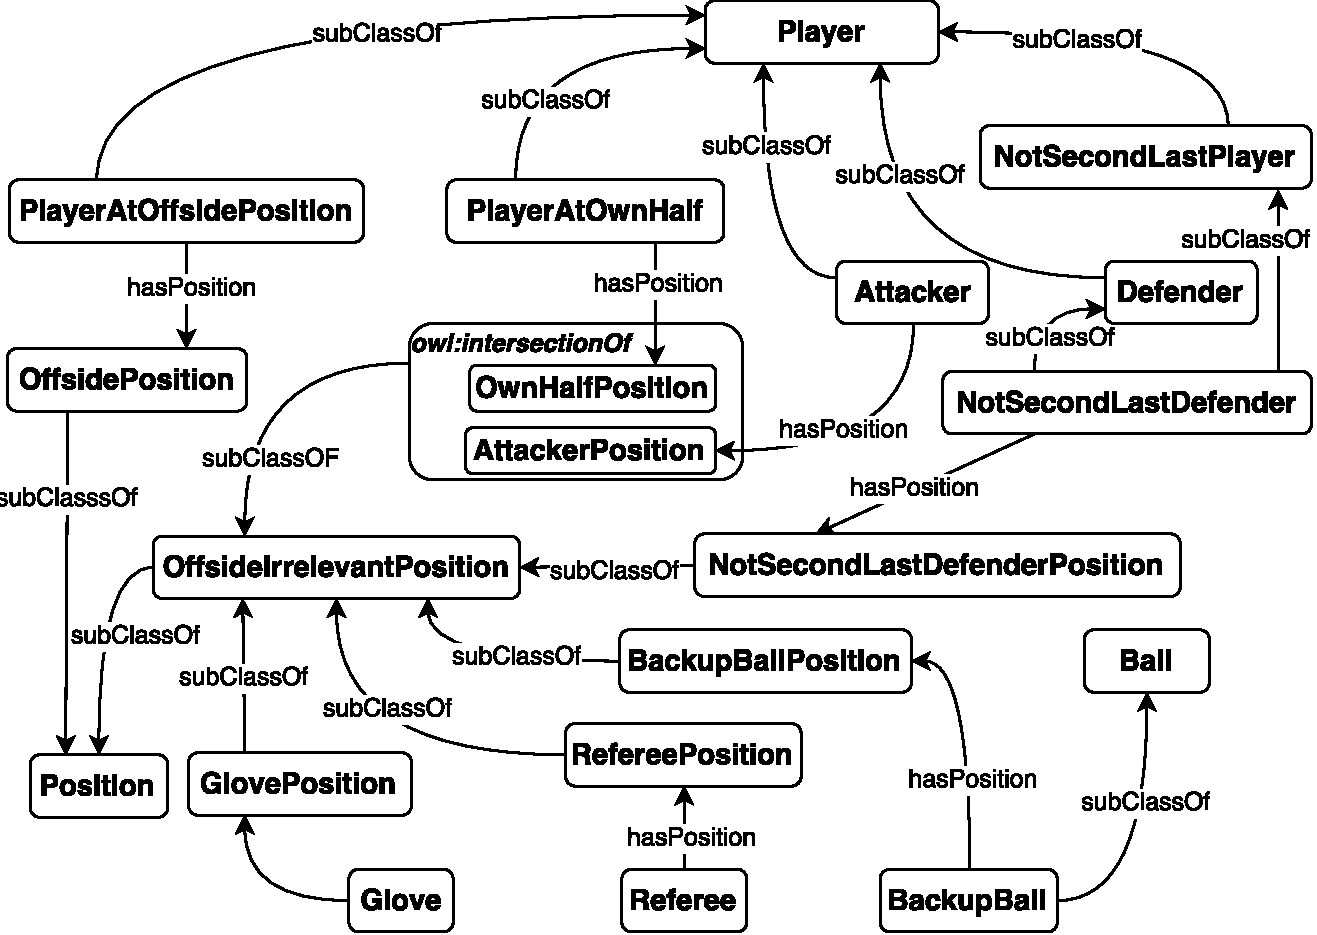
\includegraphics[width=5in]{img/5-qronto}
	\caption{\textbf{Soccer Offence Query Relevance Ontology}}
	\label{fig:dlonto}
\end{figure}

Figure \ref{fig:dlonto} illustrates the query relevance ontology. 
This use case is scoped to answer the question of who commits an offside offence. 
If a data item does not contain offside offence information, there is no need to execute the query on it. 
The purpose of this ontology module is to identify and eliminate the irrelevant data by leveraging semantics to ask another question (an example is in Listing 5.2) of what the offside irrelevant positions are prior to executing the offside query.
For the data set of this use case, all ball positions, referee positions, goalkeeper glove positions and player's positions are present. 
In this ontology, glove's position \textbf{GlovePosition}, referee's position \textbf{RefereePosition}, back up balls' positions \textbf{BackupBallPosition}, positions of defenders who are not the second last player \textbf{NotSecondLastDefenderPosition}, positions of attackers who are in their own half (\textit{owl:intersectionOf} (\textbf{AttackerPosition} \textit{and} \textbf{OwnHalfPosition})) are all offside irrelevant positions \textbf{OffsideIrrelevantPosition}, which means that these types of data will not provide necessary information to the query at hand, thus can be filtered out before the target query execution. 
%
\subsection{Data Annotation}
The original streaming data comes in comma-delimited format with the schema as  ($sid, ts, x, y, z, \left|v\right|, \left|a\right|, v_{x}, v_{y}, v_{z}, a_{x}, a_{y}, a_{z}$), where $sid$ denotes the sensor ID, $ts$ denotes the generation timestamp in pico-seconds, $(x, y, z)$ denotes a sensor coordinate in 3D space, and $(\left|v\right|, \left|a\right|, v_{x}, v_{y}, v_{z}, a_{x}, a_{y}, a_{z})$ denotes sensor velocity, acceleration and their directions.
In this use case, $(sid, ts, x, y, z)$ will be used.

Each shin-guard of a player is installed with a sensor.
A player's position is obtained by averaging his sensor coordinates.
With the coordinates of the field markings, and player/ball positions, position coordinates can be calculated to get information, such as which balls are on or off the field or which players are in or not in their own half, etc. 
Euclidean distance is used to determine if there is an active play of either a ball-touch or an opponent-challenge.
All players are ranked according to their distances from the ball in play.
The Player-ball distance is not based on the averaged player coordinate, but the actual left and right shinguard sensor to ball sensor. 
This increases the annotation accuracy. 
That a player touches the ball is determined when he has the nearest distance to the ball that is less than 0.6 meter.
An opponent-challenge scenario is also determined when opponent-opponent distance is less than 0.6 meter.
Once a ball-touch is detected, all attacking players' distance from the defender goal line and the ball will be calculated.
Each player's distance from his own goal line will also be calculated so as to determine who is the second-last player of each team. 
The data is then annotated as in Table \ref{tab:dat}.

\begin{table}[!htbp]
    \centering
	\caption{\textbf{Data Annotation Table}}
    \label{tab:dat}
    \begin{tabular}{|c|c|} \hline
        data & annotation \\ \hhline{|==|}
		\multicolumn{2}{|c|}{player annotation} \\ \hhline{|==|}
        \textit{playerX} position & \textit{:playerX :hasPosition :playerPosition\_ts} \\ \hline
        \textit{playerX} is in own half & \textit{:playerX a :PlayerInOwnHalf} \\ \hline
        \textit{playerX} is not in own half & \textit{:playerX a PlayerNotInOwnHalf} \\ \hline
        \textit{playerX} is a second-last player & \textit{:playerX a SecondLastPlayer} \\ \hline
        \textit{playerX} is not a second-last player & \textit{:playerX a NotSecondLastPlayer} \\ \hline
        \textit{playerX} touches the ball & \textit{:playerX :isInvolvedIn :ball\_touch} \\ \hline
        \multirow{2}{*}{if \textit{playerX} challenges \textit{playerY}} & \textit{:playerX :isInvolvedIn :opponent\_challenge} \\ & \textit{:playerY :isInvolvedIn :opponent\_challenge} \\ \hhline{|==|}
        \multicolumn{2}{|c|}{ball annotation} \\ \hhline{|==|}
        \textit{ballA} position & \textit{:ballA :hasPosition :ballPosition\_ts} \\ \hline
        \textit{ballA} is in the field & \textit{:ballA a :InFieldBall} \\ \hline
        \textit{ballA} is off the field & \textit{:ballA a :BackupBall} \\ \hhline{|==|}
        \multicolumn{2}{|c|}{referee \& glove annotation} \\ \hhline{|==|}
        referee position & \textit{:referee :hasPosition :refereePosition\_ts} \\ \hline
        glove position & \textit{:glove :hasPosition :glovePosition\_ts} \\ \hline
	\end{tabular}
\end{table}

%
\subsection{System Implementation}
The detection system is implemented with SSRA, where a SPARQL query in Listing 5.1 is deployed.
This query is simple, but requires Description Logic (DL) reasoning. 

The sensor frequency is high such that the amount of data entered at the system is very big. 
Thus we have leveraged systematic sampling \footnote{https://en.wikipedia.org/wiki/Systematic\_sampling (Date Last Accessed: Mar. 20, 2018)} to reduce the balls' data update frequency to 20Hz, and the players' data to 10Hz.
Sampling will not affect the result as both balls and players move only a short distance every 0.05 and 0.1 second.

\begin{lstlisting}[caption={\textbf{Offside Offence Detection Query}},basicstyle=\small]
PREFIX so:<http://tw.rpi.edu/Ontologies/2016/Soccer_Offside/>
SELECT ?player 
WHERE { ?player a so:PlayerCommitsOffsideOffence.}
\end{lstlisting}

A physical sliding window is leveraged.
According to our annotation strategy, the maximum number of unique triples is 70, which includes the ``\textit{hasPosition}'' triples from 1 referee, 16 players, 4 balls and 4 gloves, as well as a certain number of ball status triples, such as ``\textit{ball4 a InFieldBall(BackupBall)}'', and player status triples, such as ``\textit{playerA4 a SecondLastPlayer(NotSecondLastPlayer, PlayerInOwnHalf, PlayerNotInOwnHalf)}'', ``\textit{playerA4 isInvolvedIn ball\_touch(opponent\_challenge)}'', etc. 
Thus the maximum physical window size ($l_{max}$) is set to be 70.

\begin{table}[!htbp]
\centering
\caption{\textbf{Strategy Table}}
\label{tab:sct}
\begin{tabular}{|l|c|}
\hline
\multicolumn{1}{|c|}{strategy} & semantic importance priority vector \\ \hline
FE-FI-FO & $[\tau_{e}, \tau_{a}]$ \\ \hline
FE-FI-FO-25\% & $[\tau_{e}, \tau_{a}]$ \\ \hline
FE-FI-FO-50\% & $[\tau_{e}, \tau_{a}]$ \\ \hline
FE-FI-FO-75\% & $[\tau_{e}, \tau_{a}]$ \\ \hline
QR-FE-FI-FO & $[qrf, \tau_{e}, \tau_{a}]$ \\ \hline
QR-FE-FI-FO-25\% & $[qrf, \tau_{e}, \tau_{a}]$ \\ \hline
QR-FE-FI-FO-50\% & $[qrf, \tau_{e}, \tau_{a}]$ \\ \hline
QR-FE-FI-FO-75\% & $[qrf, \tau_{e}, \tau_{a}]$ \\ \hline
FE-LFU-FO & $[\tau_{e}, f_{qp}]$ \\ \hline
FE-LFU-FO-25\% & $[\tau_{e}, f_{qp}]$ \\ \hline
FE-LFU-FO-50\% & $[\tau_{e}, f_{qp}]$ \\ \hline
FE-LFU-FO-75\% & $[\tau_{e}, f_{qp}]$ \\ \hline
QR-FE-LFU-FO & $[qrf, \tau_{e}, f_{qp}]$ \\ \hline
QR-FE-LFU-FO-25\% & $[qrf, \tau_{e}, f_{qp}]$ \\ \hline
QR-FE-LFU-FO-50\% & $[qrf, \tau_{e}, f_{qp}]$ \\ \hline
QR-FE-LFU-FO-75\% & $[qrf, \tau_{e}, f_{qp}]$ \\ \hline
FE-LRU-FO & $[\tau_{e}, \tau_{qp}]$ \\ \hline
FE-LRU-FO-25\% & $[\tau_{e}, \tau_{qp}]$ \\ \hline
FE-LRU-FO-50\% & $[\tau_{e}, \tau_{qp}]$ \\ \hline
FE-LRU-FO-75\% & $[\tau_{e}, \tau_{qp}]$ \\ \hline
QR-FE-LRU-FO & $[qrf, \tau_{e}, f_{qp}]$ \\ \hline
QR-FE-LRU-FO-25\% & $[qrf, \tau_{e}, f_{qp}]$ \\ \hline
QR-FE-LRU-FO-50\% & $[qrf, \tau_{e}, f_{qp}]$ \\ \hline
QR-FE-LRU-FO-75\% & $[qrf, \tau_{e}, f_{qp}]$ \\ \hline
\end{tabular}
\end{table}

For this use case, semantic importance aspects including $\tau_{a}$, $\tau_{e}$, $qrf$, $f_{qp}$, and $\tau_{qp}$ are chosen to form the strategies shown in Table \ref{tab:sct}. 
All strategies labeled with QR perform query relevance filtering (Listing 5.2) before executing the offside query in Listing 5.1. 
The percentage after each strategy indicates the percentage of $l_{max}$. 
For example, FE-LFU-FO-25\% means FE-LFU-FO strategy is performed in a window with 25\% of $l_{max}$, which is 70 $\times$ 0.25 = 17 data items.

This use case uses a different report policy that is not included in the SECRET model \cite{botan2010secret}.
It is named as ``on user-specified condition''. 
Specifically, the offside query is fired whenever a different player touches the ball.
It is important for this use case to execute the query based on ball touches, as all the status of the players will likely be changed upon each ball touch. 
Executing query based on time will potentially allow inconsistent data items, such as a player is both an attacker and defender. 

\begin{figure}[!htbp]
	\centering
	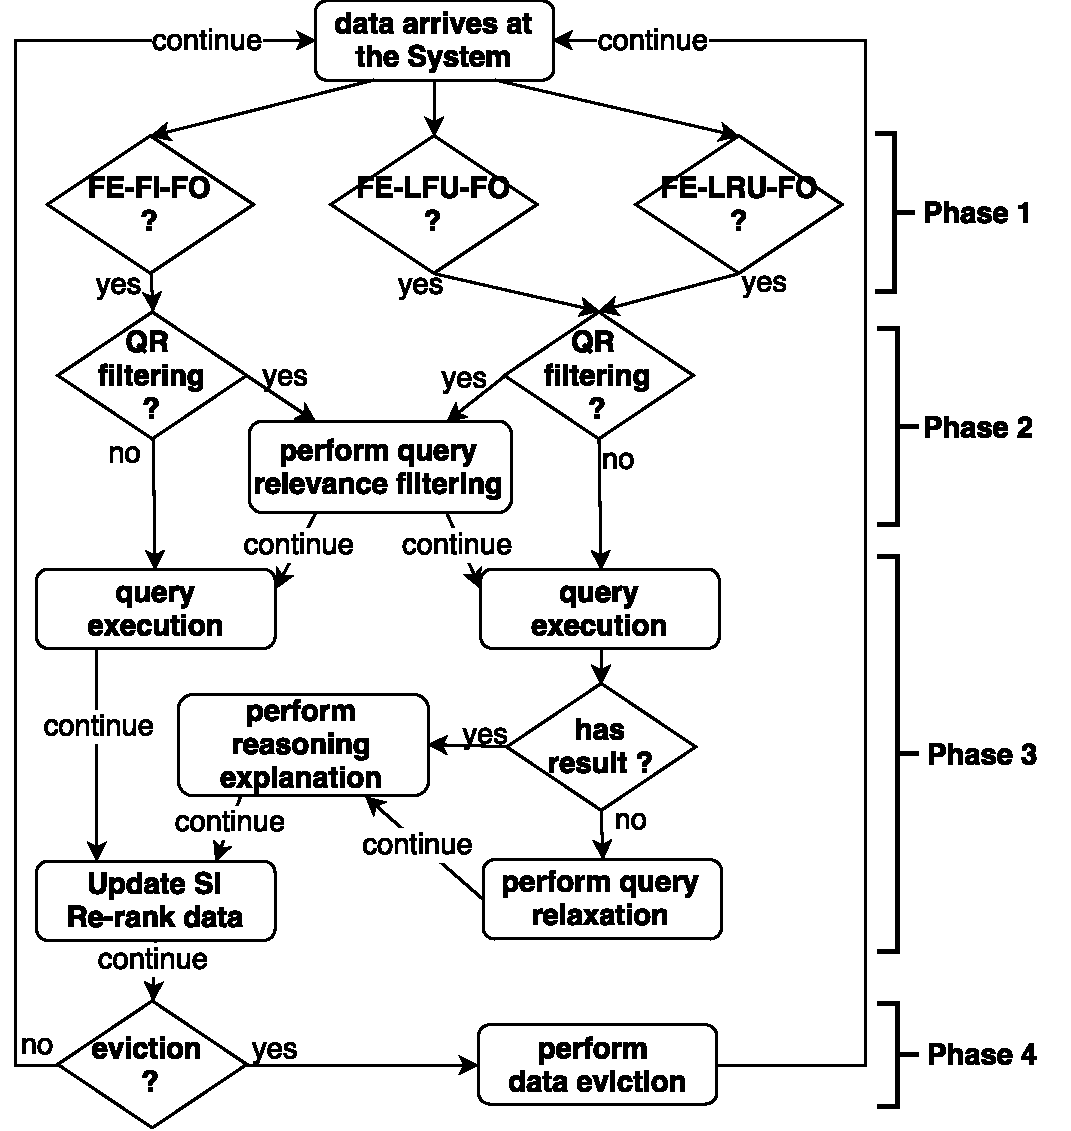
\includegraphics[width=5in]{img/5-strategyexe.pdf}
	\caption{\textbf{Strategy Execution Flowchart}}
	\label{fig:strExe}
\end{figure}

The strategies executed are shown by the paths through the graph in Figure \ref{fig:strExe}. 
Depending on the priority vector, Phase 1 is the selection of a base strategy family to run. 
If the SI priority vector has the first element of ``$qrf$'', the QR filtering is performed by executing the query in Listing 5.2.

Phase 3 executes the offside query when a new player touches the ball.
If current strategy is in the *-FI-FO family, the system will go ahead to update the semantic importance and re-rank the data. 
If the current strategy is in the *-LRU/LFU-FO family, the system will need to check if the offside query returns any results.
If there are results, reasoning explanation is performed to track all the triples that contribute to the query.
If no result, schema-aware query relaxation \cite{hurtado2008query} will be performed to increase the scope of the query.
For example, if the query returns no answer, the system continues to ask who touches the ball, who is the second-last player, who is nearer to the opponents' goal line than whom, etc. 
Listing 5.3 shows a relaxed query.

\begin{lstlisting}[caption={\textbf{Query Relevance Filtering Query}},basicstyle=\small]
PREFIX so:<http://tw.rpi.edu/Ontologies/2016/Soccer_Offside/>
SELECT ?player 
WHERE { 
    ?position a so:OffsideIrrevelantPosition.
}
\end{lstlisting}

\begin{lstlisting}[caption={\textbf{A Relaxed Query Example}},basicstyle=\small]
PREFIX so:<http://tw.rpi.edu/Ontologies/2016/Soccer_Offside/>
SELECT ?s ?p ?o
WHERE {
	?s a so:SecondLastPlayer.
	bind(IRI(rdf:type) as ?p).
	bind(IRI(so:SecondLastPlayer) as ?o)
}
\end{lstlisting}

Being able to preserve some partial necessary data and wait until the others arrive, and then answer the query, is a key feature for *-LRU/LFU-FO families enabled by $\tau_{qp}$ and $f_{qp}$.
It also explains why they have higher accuracy -- the offside offence judgement requires the window to preserve earlier information (player in offside position at the moment his teammate passes the ball) until later information (the player involved in an active play) arrives.
After query relaxation, semantic importance priority vectors will be updated, and the window data will be re-ranked. 
Next, the system checks the percentage of $l_{max}$ which the strategy comes with, and performs data eviction accordingly. 
Obviously, the use case expects that FE-FI-FO, QR-FE-FI-FO, FE-LFU-FO, QR-FE-LFU-FO, FE-LRU-FO and QR-FE-LRU-FO with $l_{max}$ will perform equally well in accuracy. 
%
\subsection{Evaluation}
Table \ref{tab:ev} presents both the referee and system offside judging results.
Table \ref{tb:rp} and \ref{tb:accuracy} show the averaged running performance and accuracy for each strategy family, respectively.  
Accuracy is computed by counting a correct answer only when referee gives \textcolor{blue}{\newmoon} and system gives \newmoon, or when referee gives \textcolor{blue}{\texttimes} and system gives \texttimes. 
For example, we calculate FE-FI-FO-25\% accuracy as 11/20 = 0.55 because it gives 11 correct results out of the total 20 cases.

\begin{table}[!htbp]
	\scriptsize
	\centering
	\caption{\textbf{Offside Detection Results}}
	\label{tab:ev}
	\begin{tabular}{|l|c|c|c|c|c|c|c|c|c|c|} \hline
Time&2:53&4:26&7:04&12:21&12:44&15:28&20:40&21:11&22:07&23:04\\ \hhline{|=|=|=|=|=|=|=|=|=|=|=|}
\textcolor{blue}{Referee}&\textcolor{blue}{\texttimes}&\textcolor{blue}{\newmoon}&\textcolor{blue}{\newmoon}&\textcolor{blue}{\texttimes}&\textcolor{blue}{\texttimes}&\textcolor{blue}{\newmoon}&\textcolor{blue}{\newmoon}&\textcolor{blue}{\newmoon}&\textcolor{blue}{\texttimes}&\textcolor{blue}{\texttimes}\\ \hline
FE-FI-FO&\texttimes&\newmoon&\newmoon&\texttimes&\texttimes&\newmoon&\newmoon&\textcolor{red}{\texttimes}&\texttimes&\texttimes\\ \hline
FE-FI-FO-25\%&\texttimes&\textcolor{red}{\fullmoon}&\textcolor{red}{\texttimes}&\textcolor{red}{\newmoon}&\texttimes&\textcolor{red}{\fullmoon}&\textcolor{red}{\texttimes}&\textcolor{red}{\fullmoon}&\texttimes&\texttimes\\ \hline
FE-FI-FO-50\%&\texttimes&\textcolor{red}{\texttimes}&\textcolor{red}{\texttimes}&\textcolor{red}{\newmoon}&\texttimes&\textcolor{red}{\texttimes}&\textcolor{red}{\texttimes}&\textcolor{red}{\texttimes}&\texttimes&\texttimes\\ \hline
FE-FI-FO-75\%&\texttimes&\textcolor{red}{\texttimes}&\textcolor{red}{\texttimes}&\texttimes&\texttimes&\textcolor{red}{\texttimes}&\textcolor{red}{\texttimes}&\textcolor{red}{\texttimes}&\texttimes&\texttimes\\ \hline
QR-FE-FI-FO&\texttimes&\newmoon&\newmoon&\texttimes&\texttimes&\newmoon&\newmoon&\textcolor{red}{\texttimes}&\texttimes&\texttimes\\ \hline
QR-FE-FI-FO-25\%&\texttimes&\textcolor{red}{\fullmoon}&\textcolor{red}{\texttimes}&\textcolor{red}{\newmoon}&\texttimes&\textcolor{red}{\fullmoon}&\textcolor{red}{\texttimes}&\textcolor{red}{\fullmoon}&\texttimes&\texttimes\\ \hline
QR-FE-FI-FO-50\%&\texttimes&\textcolor{red}{\texttimes}&\textcolor{red}{\texttimes}&\textcolor{red}{\newmoon}&\texttimes&\textcolor{red}{\texttimes}&\textcolor{red}{\texttimes}&\textcolor{red}{\texttimes}&\texttimes&\texttimes\\ \hline
QR-FE-FI-FO-75\%&\texttimes&\textcolor{red}{\texttimes}&\textcolor{red}{\texttimes}&\texttimes&\texttimes&\textcolor{red}{\texttimes}&\textcolor{red}{\texttimes}&\textcolor{red}{\texttimes}&\texttimes&\texttimes\\ \hline
FE-LFU-FO&\texttimes&\newmoon&\newmoon&\texttimes&\texttimes&\newmoon&\newmoon&\textcolor{red}{\texttimes}&\texttimes&\texttimes\\ \hline
FE-LFU-FO-25\%&\texttimes&\newmoon&\newmoon&\texttimes&\texttimes&\newmoon&\newmoon&\textcolor{red}{\fullmoon}&\texttimes&\texttimes\\ \hline
FE-LFU-FO-50\%&\texttimes&\newmoon&\newmoon&\texttimes&\texttimes&\newmoon&\newmoon&\textcolor{red}{\fullmoon}&\texttimes&\texttimes\\ \hline
FE-LFU-FO-75\%&\texttimes&\newmoon&\newmoon&\texttimes&\texttimes&\newmoon&\newmoon&\textcolor{red}{\texttimes}&\texttimes&\texttimes\\ \hline
QR-FE-LFU-FO&\texttimes&\newmoon&\newmoon&\texttimes&\texttimes&\newmoon&\newmoon&\textcolor{red}{\texttimes}&\texttimes&\texttimes\\ \hline
QR-FE-LFU-FO-25\%&\texttimes&\newmoon&\newmoon&\texttimes&\texttimes&\newmoon&\newmoon&\textcolor{red}{\fullmoon}&\texttimes&\texttimes\\ \hline
QR-FE-LFU-FO-50\%&\texttimes&\newmoon&\newmoon&\texttimes&\texttimes&\newmoon&\newmoon&\textcolor{red}{\fullmoon}&\texttimes&\texttimes\\ \hline
QR-FE-LFU-FO-75\%&\texttimes&\newmoon&\newmoon&\texttimes&\texttimes&\newmoon&\newmoon&\textcolor{red}{\fullmoon}&\texttimes&\texttimes\\ \hline
FE-LRU-FO&\texttimes&\newmoon&\newmoon&\texttimes&\texttimes&\newmoon&\newmoon&\textcolor{red}{\texttimes}&\texttimes&\texttimes\\ \hline
FE-LRU-FO-25\%&\texttimes&\newmoon&\newmoon&\texttimes&\texttimes&\newmoon&\newmoon&\textcolor{red}{\fullmoon}&\texttimes&\texttimes\\ \hline
FE-LRU-FO-50\%&\texttimes&\newmoon&\newmoon&\texttimes&\texttimes&\newmoon&\newmoon&\textcolor{red}{\fullmoon}&\texttimes&\texttimes\\ \hline
FE-LRU-FO-75\%&\texttimes&\newmoon&\newmoon&\texttimes&\texttimes&\newmoon&\newmoon&\textcolor{red}{\fullmoon}&\texttimes&\texttimes\\ \hline
QR-FE-LRU-FO&\texttimes&\newmoon&\newmoon&\texttimes&\texttimes&\newmoon&\newmoon&\textcolor{red}{\texttimes}&\texttimes&\texttimes\\ \hline
QR-FE-LRU-FO-25\%&\texttimes&\newmoon&\newmoon&\texttimes&\texttimes&\newmoon&\newmoon&\textcolor{red}{\fullmoon}&\texttimes&\texttimes\\ \hline
QR-FE-LRU-FO-50\%&\texttimes&\newmoon&\newmoon&\texttimes&\texttimes&\newmoon&\newmoon&\textcolor{red}{\fullmoon}&\texttimes&\texttimes\\ \hline
QR-FE-LRU-FO-75\%&\texttimes&\newmoon&\newmoon&\texttimes&\texttimes&\newmoon&\newmoon&\textcolor{red}{\fullmoon}&\texttimes&\texttimes\\ \hhline{===========}
Time&30:52&40:30&40:45&42:16&47:38&50:25&51:43&54:46&58:11&58:24 \\  \hhline{|=|=|=|=|=|=|=|=|=|=|=|}
\textcolor{blue}{Referee}&\textcolor{blue}{\texttimes}&\textcolor{blue}{\texttimes}&\textcolor{blue}{\newmoon}&\textcolor{blue}{$\otimes$}&\textcolor{blue}{$\otimes$}&\textcolor{blue}{$\otimes$}&\textcolor{blue}{$\otimes$}&\textcolor{blue}{\newmoon}&\textcolor{blue}{$\otimes$}&\textcolor{blue}{\texttimes}  \\ \hline
FE-FI-FO&\texttimes&\texttimes&\newmoon&\texttimes&\texttimes&\texttimes&\texttimes&\textcolor{red}{\texttimes}&\newmoon&\texttimes  \\ \hline
FE-FI-FO-25\%&\texttimes&\texttimes&\textcolor{red}{\texttimes}&\texttimes&\texttimes&\texttimes&\texttimes&\textcolor{red}{\fullmoon}&\texttimes&\textcolor{red}{\newmoon} \\ \hline
FE-FI-FO-50\%&\texttimes&\texttimes&\textcolor{red}{\texttimes}&\texttimes&\texttimes&\texttimes&\texttimes&\textcolor{red}{\fullmoon}&\texttimes&\textcolor{red}{\newmoon} \\ \hline
FE-FI-FO-75\%&\texttimes&\texttimes&\textcolor{red}{\texttimes}&\texttimes&\texttimes&\texttimes&\texttimes&\textcolor{red}{\texttimes}&\texttimes&\texttimes  \\ \hline
QR-FE-FI-FO&\texttimes&\texttimes&\newmoon&\texttimes&\texttimes&\texttimes&\texttimes&\textcolor{red}{\texttimes}&\newmoon&\texttimes  \\ \hline
QR-FE-FI-FO-25\%&\texttimes&\texttimes&\textcolor{red}{\texttimes}&\texttimes&\texttimes&\texttimes&\texttimes&\textcolor{red}{\fullmoon}&\texttimes&\textcolor{red}{\newmoon} \\ \hline
QR-FE-FI-FO-50\%&\texttimes&\texttimes&\textcolor{red}{\texttimes}&\texttimes&\texttimes&\texttimes&\texttimes&\textcolor{red}{\texttimes}&\texttimes&\textcolor{red}{\newmoon} \\ \hline
QR-FE-FI-FO-75\%&\texttimes&\texttimes&\textcolor{red}{\texttimes}&\texttimes&\texttimes&\texttimes&\texttimes&\textcolor{red}{\texttimes}&\texttimes&\texttimes  \\ \hline
FE-LFU-FO&\texttimes&\texttimes&\newmoon&\texttimes&\texttimes&\texttimes&\texttimes&\textcolor{red}{\texttimes}&\newmoon&\texttimes  \\ \hline
FE-LFU-FO-25\%&\texttimes&\texttimes&\newmoon&\texttimes&\texttimes&\texttimes&\texttimes&\textcolor{red}{\texttimes}&\newmoon&\texttimes  \\ \hline
FE-LFU-FO-50\%&\texttimes&\texttimes&\newmoon&\texttimes&\texttimes&\texttimes&\texttimes&\textcolor{red}{\texttimes}&\newmoon&\texttimes  \\ \hline
FE-LFU-FO-75\%&\texttimes&\texttimes&\newmoon&\texttimes&\texttimes&\texttimes&\texttimes&\textcolor{red}{\texttimes}&\newmoon&\texttimes  \\ \hline
QR-FE-LFU-FO&\texttimes&\texttimes&\newmoon&\texttimes&\texttimes&\texttimes&\texttimes&\textcolor{red}{\texttimes}&\newmoon&\texttimes  \\ \hline
QR-FE-LFU-FO-25\%&\texttimes&\texttimes&\newmoon&\texttimes&\texttimes&\texttimes&\texttimes&\textcolor{red}{\texttimes}&\newmoon&\texttimes  \\ \hline
QR-FE-LFU-FO-50\%&\texttimes&\texttimes&\newmoon&\texttimes&\texttimes&\texttimes&\texttimes&\textcolor{red}{\texttimes}&\newmoon&\texttimes  \\ \hline
QR-FE-LFU-FO-75\%&\texttimes&\texttimes&\newmoon&\texttimes&\texttimes&\texttimes&\texttimes&\textcolor{red}{\texttimes}&\newmoon&\texttimes  \\ \hline
FE-LRU-FO&\texttimes&\texttimes&\newmoon&\texttimes&\texttimes&\texttimes&\texttimes&\textcolor{red}{\texttimes}&\newmoon&\texttimes  \\ \hline
FE-LRU-FO-25\%&\texttimes&\texttimes&\newmoon&\texttimes&\texttimes&\texttimes&\texttimes&\textcolor{red}{\texttimes}&\newmoon&\texttimes  \\ \hline
FE-LRU-FO-50\%&\texttimes&\texttimes&\newmoon&\texttimes&\texttimes&\texttimes&\texttimes&\textcolor{red}{\texttimes}&\newmoon&\texttimes  \\ \hline
FE-LRU-FO-75\%&\texttimes&\texttimes&\newmoon&\texttimes&\texttimes&\texttimes&\texttimes&\textcolor{red}{\texttimes}&\newmoon&\texttimes  \\ \hline
QR-FE-LRU-FO&\texttimes&\texttimes&\newmoon&\texttimes&\texttimes&\texttimes&\texttimes&\textcolor{red}{\texttimes}&\newmoon&\texttimes  \\ \hline
QR-FE-LRU-FO-25\%&\texttimes&\texttimes&\newmoon&\texttimes&\texttimes&\texttimes&\texttimes&\textcolor{red}{\texttimes}&\newmoon&\texttimes  \\ \hline
QR-FE-LRU-FO-50\%&\texttimes&\texttimes&\newmoon&\texttimes&\texttimes&\texttimes&\texttimes&\textcolor{red}{\texttimes}&\newmoon&\texttimes  \\ \hline
QR-FE-LRU-FO-75\%&\texttimes&\texttimes&\newmoon&\texttimes&\texttimes&\texttimes&\texttimes&\textcolor{red}{\texttimes}&\newmoon&\texttimes  \\ \hline
	\end{tabular}
	\begin{tablenotes}
 		\item \textcolor{blue}\newmoon:referee confirmed offside offence
        \item \textcolor{blue}\texttimes:referee confirmed no offside offence
        \item \textcolor{blue}{$\otimes$}:referee unsure so no flag 
        \item \newmoon:system true-positive judgment 
        \item \texttimes:system true-negative judgment
        \item \textcolor{red}\newmoon:system false-positive judgment 
        \item \textcolor{red}\texttimes:system false-negative judgment 
        \item \textcolor{red}\fullmoon:system confirmed judgment but with wrong judging foundation
    \end{tablenotes}
\end{table}

From these tables, it can be observed that among all the strategies: 
(1) the *-FI-FO family intakes and evicts data the fastest, but has the slowest execution time and is more error-prone, especially when the window size is smaller; 
(2) *-LFU-FO and *-LRU-FO families both have slower throughput and eviction than *-FI-FO family, and require extra time to explain the inference, but maintain a good accuracy even if the window size shrinks; 
(3) the QR-* family's query and execution time is the fastest; 
(4) the results of FE-FI-FO, QR-FE-FI-FO, FE-LFU-FO, QR-FE-LFU-FO, FE-LRU-FO and QR-FE-LRU-FO at $l_{max}$ are all identical, which validates our expectations above;
(5) the use case situations at 21:11 and 54:46 makes all strategies fail; 
(6) no consensus is reached by all strategies for the unsure case at 58:11. 

The reason for *-FI-FO family accuracy performance is that, when equipped with $l_{max}$, FE-FI-FO and QR-FE-FI-FO evict only expired\slash domain irrelevant data, so all unexpired\slash relevant data are preserved.
However, when $l$ shrinks, decisions to delete valid data from the window have to be made. 
According to the semantic importance priority vector [$\tau_{e}, \tau_{a}$], if a data item is not expired, the one with the earliest arrival timestamp is ranked at the bottom, thus evicted. 
If the time interval/triple counts between the data of offside position and data of active play is larger than the deployed window size, it is impossible to have both of them in the window at the same time, therefore a false-negative (\textcolor{red}{\texttimes}) result will be given.
This situation also causes a false-positive (\textcolor{red}{\newmoon}) or wrong foundation (\textcolor{red}{\fullmoon}) judgment. 

Figure \ref{fig:fpa}.(a) shows that at the moment Player A2 touches the ball, Player B4 is the second-last defender; Player A7 is not in offside position.
So Player A7 does not commit an offside offence when he touches the ball.
According to our data annotation process, since Player A7 uses his left back heel to touch the ball in Figure \ref{fig:fpa}.(b), his left shin-guard sensor is nearer to the defender's goal line than both the ball and Player B1, thus Player A7 is annotated as ``\textit{playerA7 isNearerToDefenderGoalLineThan ball}''; ``\textit{playerA7 isNearerToDefenderGoalLineThan playerB1}''.
Although it is only one touch, this ball-touch is detected 361 times based on the distance between Player A7's shin-guard sensor and ball sensor.
For each ball-touch detection, the annotation strategy will detect if ``\textit{isNearerToDefenderGoalLineThan}'' information exits and output it if it exists.
Between two ball-touch triples, there are usually some triples as shown in Listing 5.4. 

\begin{lstlisting}[caption={\textbf{Ball Touch Annotation}},basicstyle=\small]
1. playerA7 isInvolvedIn ball_touch
2. playerB1 a SecondLastPlayer
3. playerA7 isNearerToDefenderGoalLineThan playerB1
4. playerA7 isNearerToDefenderGoalLineThan ball8
   ...
5. ball8 a InFieldBall
6. playerA7 isInvolvedIn ball_touch
\end{lstlisting}

Triple \#1 in Listing 5.4 is easily evicted by FE-FI-FO with a small $l$, which loses the ball-toucher information.
When Triple \#6 arrives, the system thinks this is a new ball toucher, thus the query is executed.
Because all necessary data(Triple \#2, 3, 4, 5 \& 6) is present, a false-positive result is returned.
The reason why FE-FI-FO, QR-FE-FI-FO, and QR-FE-FI-FO-75\% return correct judgments is that their window size is large enough to hold the triples between two adjacent ball-toucher triples, thus the in-window ball-toucher triple only needs to update its generation timestamp, rather than being evicted.
This example also illustrates the importance to fire query upon ball-touch events, not time. 

However, for *-LFU/LRU-FO families, the mechanism is different. 
They can use query participation aspect to collect more important data via either query execution or query relaxation, thus Triple \#1 will always be preserved to avoid executing the offside query again and again, till a different ball-toucher arrives.
For \textcolor{red}{\fullmoon} result, its cause is the same as the false negative judgment -- the *-FI-FO family with small $l$ cannot preserve the offside position status of Player A6 in Figure \ref{fig:fpa}.(c), but uses the offside position status in Figure \ref{fig:fpa}.(d), which is based on a wrong judging foundation.
As a matter of fact, what happens during 21:11 to 21:13 is that, ball is passed from Player A1 to Player A6, while Player B1 tries really hard to steal the ball, but fails to change the ball's trajectory. 
Since Player B1 and the ball distance is very close (smaller than 0.6m) when he reaches out his feet, the system thinks there is an offensive transition. 
Thus all the yellow teammates become defenders. 
However, as Player A6 touches the ball, the system thinks there is another offensive transition happens. 
Thus at this moment, which is shown in Figure \ref{fig:fpa}.(d), Player A6 is at the offside position, is an attacker, touches the ball. 
So the system reports that this is an offside offence. 
Some strategies produce \textcolor{red}{\fullmoon} because of the window size is small, as well as two offensive transitions that can expire the players' status data, so that the window cannot hold the correct offside judging foundation status happening at Figure \ref{fig:fpa}.(c). 
In sum, that Player A6 commits an offside offence is true, but this judgment should be made upon the offside position in Figure \ref{fig:fpa}.(c), not \ref{fig:fpa}.(d)

\begin{figure}[!htbp]
	\centering
	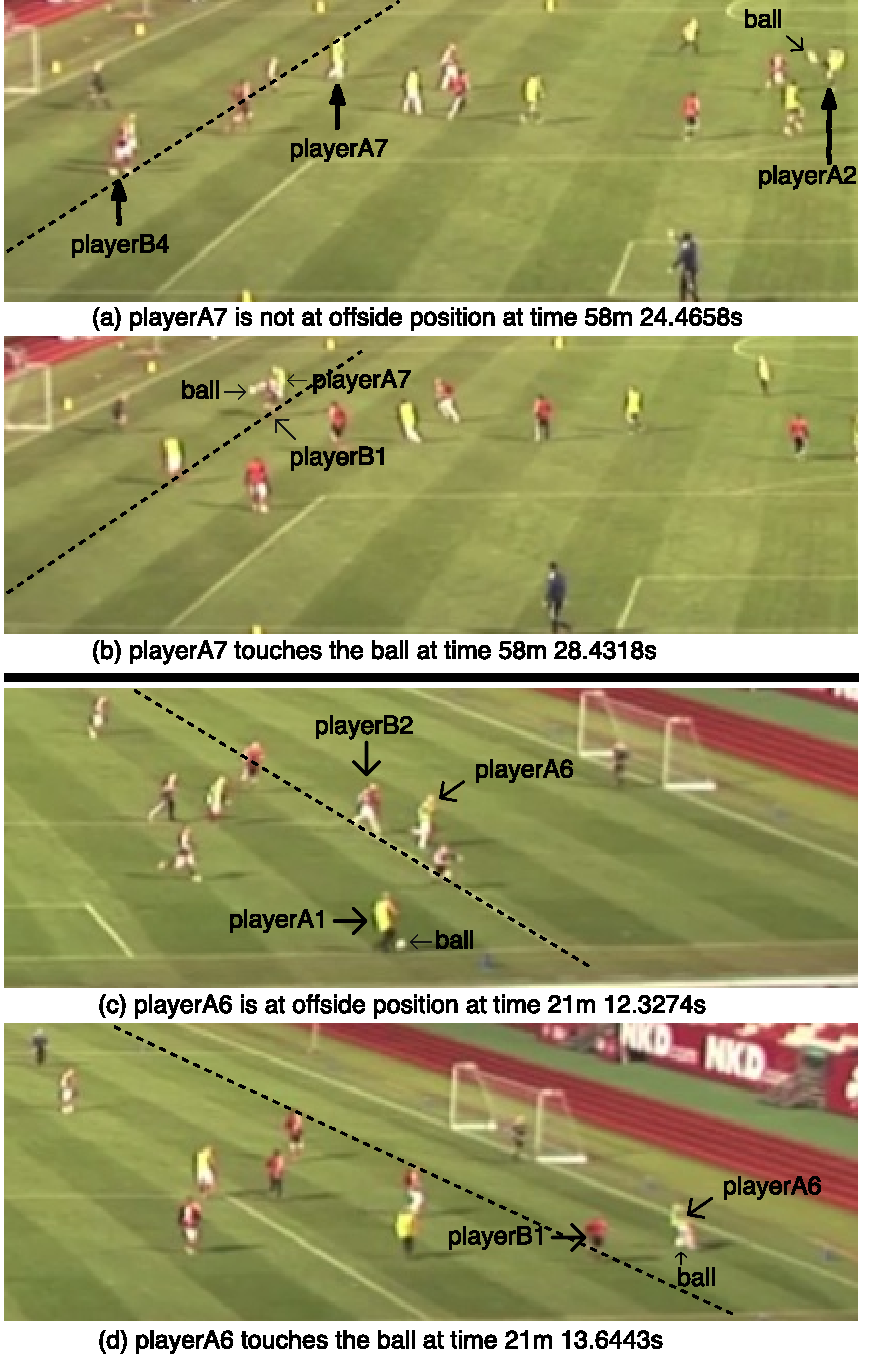
\includegraphics[width=5in]{img/5-fpa}
	\caption{\textbf{False-positive \& Wrong Foundation Judging Analysis}}
	\label{fig:fpa}
\end{figure}

In addition to the results following the process described above, we reviewed the data for the 54:48 case more closely. 
In this case, the nearest player to ball is always Player B4 from 54:44 to 54:46.
However, the distance between Player B4 to ball increases from 59.9 cm to 140 cm, and the video shows that Player B4 touches the ball during that time.
Therefore, we believe that Player B4's sensor failed and lost his position during that time.
This potential sensor failure is not mentioned in DEBS 2013 grand challenge \cite{mutschler2013debs}. 

\begin{table}[!htbp]
\centering
\caption{\textbf{Strategy Running Performance}}
\label{tb:rp}
\begin{tabular}{|l||c|c|c|c|}
\hline
 & *-FI-FO & *-LFU-FO & *-LRU-FO & QR-* \\ \hhline{|=#=|=|=|=|}
Throughput (\#/s) & 497.48 & 306.48 & 328.21 & 381.81 \\ \hline
Eviction Rate (\#/s) & 130.55 & 120.32 & 114.63 & 123.31 \\ \hline
Query Time (s) & 0.34 & 0.30 & 0.33 & 0.18 \\ \hline
Explanation Time (s) & - & 0.03 & 0.03 & 0.03 \\ \hline
QR filtering Time (s) & 0.63 & 0.54 & 0.61 & 0.60 \\ \hhline{|=#=|=|=|=|}
Total Execution Time (s) & 0.97 & 0.87 & 0.97 & 0.81 \\ \hline
\end{tabular}
\end{table}

\begin{table}[!htbp]
\centering
\caption{\textbf{Strategy Accuracy Analysis}}
\label{tb:accuracy}
\begin{tabular}{|c||c|c|c|c|}
\hline
window size $l$ & *-FI-FO & *-LFU-FO & *-LRU-FO & QR-* \\ \hhline{|=#=|=|=|=|}
25\% $l_{max}$ & 0.55 & 0.90 & 0.90 & 0.80 \\ \hline
50\% $l_{max}$ & 0.55 & 0.90 & 0.90 & 0.80 \\ \hline
75\% $l_{max}$ & 0.65 & 0.90 & 0.90 & 0.83 \\ \hline
$l_{max}$ & 0.90 & 0.90 & 0.90 & 0.90 \\ \hline
\end{tabular}
\end{table}

Table \ref{tab:error} summarizes the occurrence ratios of flag errors and non-flag errors when different strategies are in use. 
In the soccer offside terminology, ``flag error'' refers to a wrong offside decision (linesman raises the flag) when there is in fact no offside offence.
Conversely, ``non-flag'' error means that no offside offence is indicated when in fact one occurs. 
The statistical counterparts of the terms ``flag error'' and ``non-flag error'' are our system's false-positive and false-negative judgments, respectively. 
It is worth mentioning that, out of the total 20 cases, there are five judgments given by the referee as ``unsure'' and thus cannot be used as ground-truth. 

\begin{table}[!htbp]
\centering
\caption{\textbf{Strategy Error Analysis}}
\label{tab:error}
\begin{tabular}{|c||c|c|c|c|l|}
\hline
 & *-FI-FO & *-LFU-FO & *-LRU-FO & QR-* & Sys. \\ \hhline{|=#=|=|=|=|=|}
flag err. & 0.07 & 0.00 & 0.00 & 0.02 & 0.02 \\ \hline
non-flag err. & 0.38 & 0.09 & 0.08 & 0.18 & 0.19 \\ \hline
\end{tabular}
\end{table}

Finally, we consider the different scenarios where each type of semantic importance can be applied. 
Generation and expiration timestamps can be applied in a system where recent data is more important, the query is simple, and does not require a history look-up. 
The throughput speed in FIFO benefits the system's real-time response. 
However, if the query is complex and requires history look-ups (as in soccer offside query answering), reasoning participation frequency and recency is better, because they can preserve historical data in the window until other complementary data arrives. 
The trade-off is a relatively lower throughput as a result of the overhead of reasoning and query explanation.
Query relevance filtering has the fastest execution time and also has the most potential to scale.
%
\section{Data Exfiltration Detection}
According to Wikipedia, ``an insider threat is a malicious threat to an organization that comes from people within the organization''\footnote{https://en.wikipedia.org/wiki/Insider\_threat (Date Last Accessed: Mar. 20, 2018)}. 
Compared to the outside threat, the organization tends to be more vulnerable when facing insider threat. 
This is because the insiders have access to the internal infrastructure, data, or network.
It is very easy for them to steal the organizational intellectual properties.
What makes it even worse is that, the insider threat is much more harder to detect than the outside threat. 
A malicious insider is defined as ``a current or former employee, contractor, or business partner who has or had authorized access to an organization's network, system or data or has intentionally exceeded or intentionally used that access in a manner that negatively affected the confidentiality, integrity, or availability of the organization's information or information systems" \cite{CERT-onto} \cite{silowash2012common}.
This use case aims to detect data exfiltration\footnote{Please refer to https://github.com/raymondino/InsiderThreat-StreamReasoningUseCase (Date Last Accessed: Mar. 20, 2018) for more details.}, a sub-category of insider threat.
%
\subsection{Background}
This use case will focus on one type of insider threat attacks, the data exfiltration. 
According to \cite{CMU-CERT}, the data exfiltration means that a malicious user employs a removable media or the Internet to remove confidential data from an organization.
An example of the data exfiltration is that the employee who finishes work usually around 5:30 PM comes back to the office very late at the night, and uses a removable disk to copy some files or upload the files into wikileaks.org.

There has already been related work that builds methods for data exfiltration. 
\cite{liu2009sidd} proposes a framework called SSID that is based on statistical and signal processing techniques to detect sensitive information distribution and stolen over the Internet. 
\cite{giani2006data} points out that the key for detecting data exfiltration is to identify the distinction between legal and illegal information communication. 
It also provides a detailed list and discussion of most known data exfiltration methods, which is very valuable to model data exfiltration. 
\cite{born2010browser} takes a different way with several novel methods of enabling data exfiltration using web browsers and the JavaScript engine, with the purpose to raise the awareness of this kind of malicious intent. 
%
\subsection{Approach}
Different from the above related work, this use case will be implemented with core notions of stream reasoning, including window and continuous processing, together with the semantic importance model and the sequential stream reasoning architecture. 
A stream reasoning system will be realized to identify and preserve all previous suspicious actions as evidence to determine data exfiltration.
Since the malicious actions can happen across arbitrary interval of time, a logical window will be leveraged. 
This poses a challenge in such a way that the bigger the window size is, the more data will be in the window to negatively affect the system responsiveness. 
In order to enable reasoning, the plan is to leverage and extend the existing insider threat ontology developed by CMU  CERT\footnote{http://www.cert.org/ (Date Last Accessed: Mar. 20, 2018)}. 
Semantic importance aspects in provenance and trustworthiness will be selected to support two window management strategies, FIFO and QR-T (query relevance - trustworthiness). 
In order to enable trustworthiness, a simple trust model is established, which will be elaborated in the following section. 
%
\subsection{Data Stream}
Real insider threat datasets are usually very organizational-sensitive and confidential, which makes it not easy to be published. 
However, \cite{glasser2013bridging} provides a synthesized streaming data set that contains four data exfiltration scenarios and provides timestamped employee actions of types including HTTP, device, login, log-off, file and email, which is shown in Figure \ref{fig:dxd}.

\begin{figure}[!htbp]
	\centering
    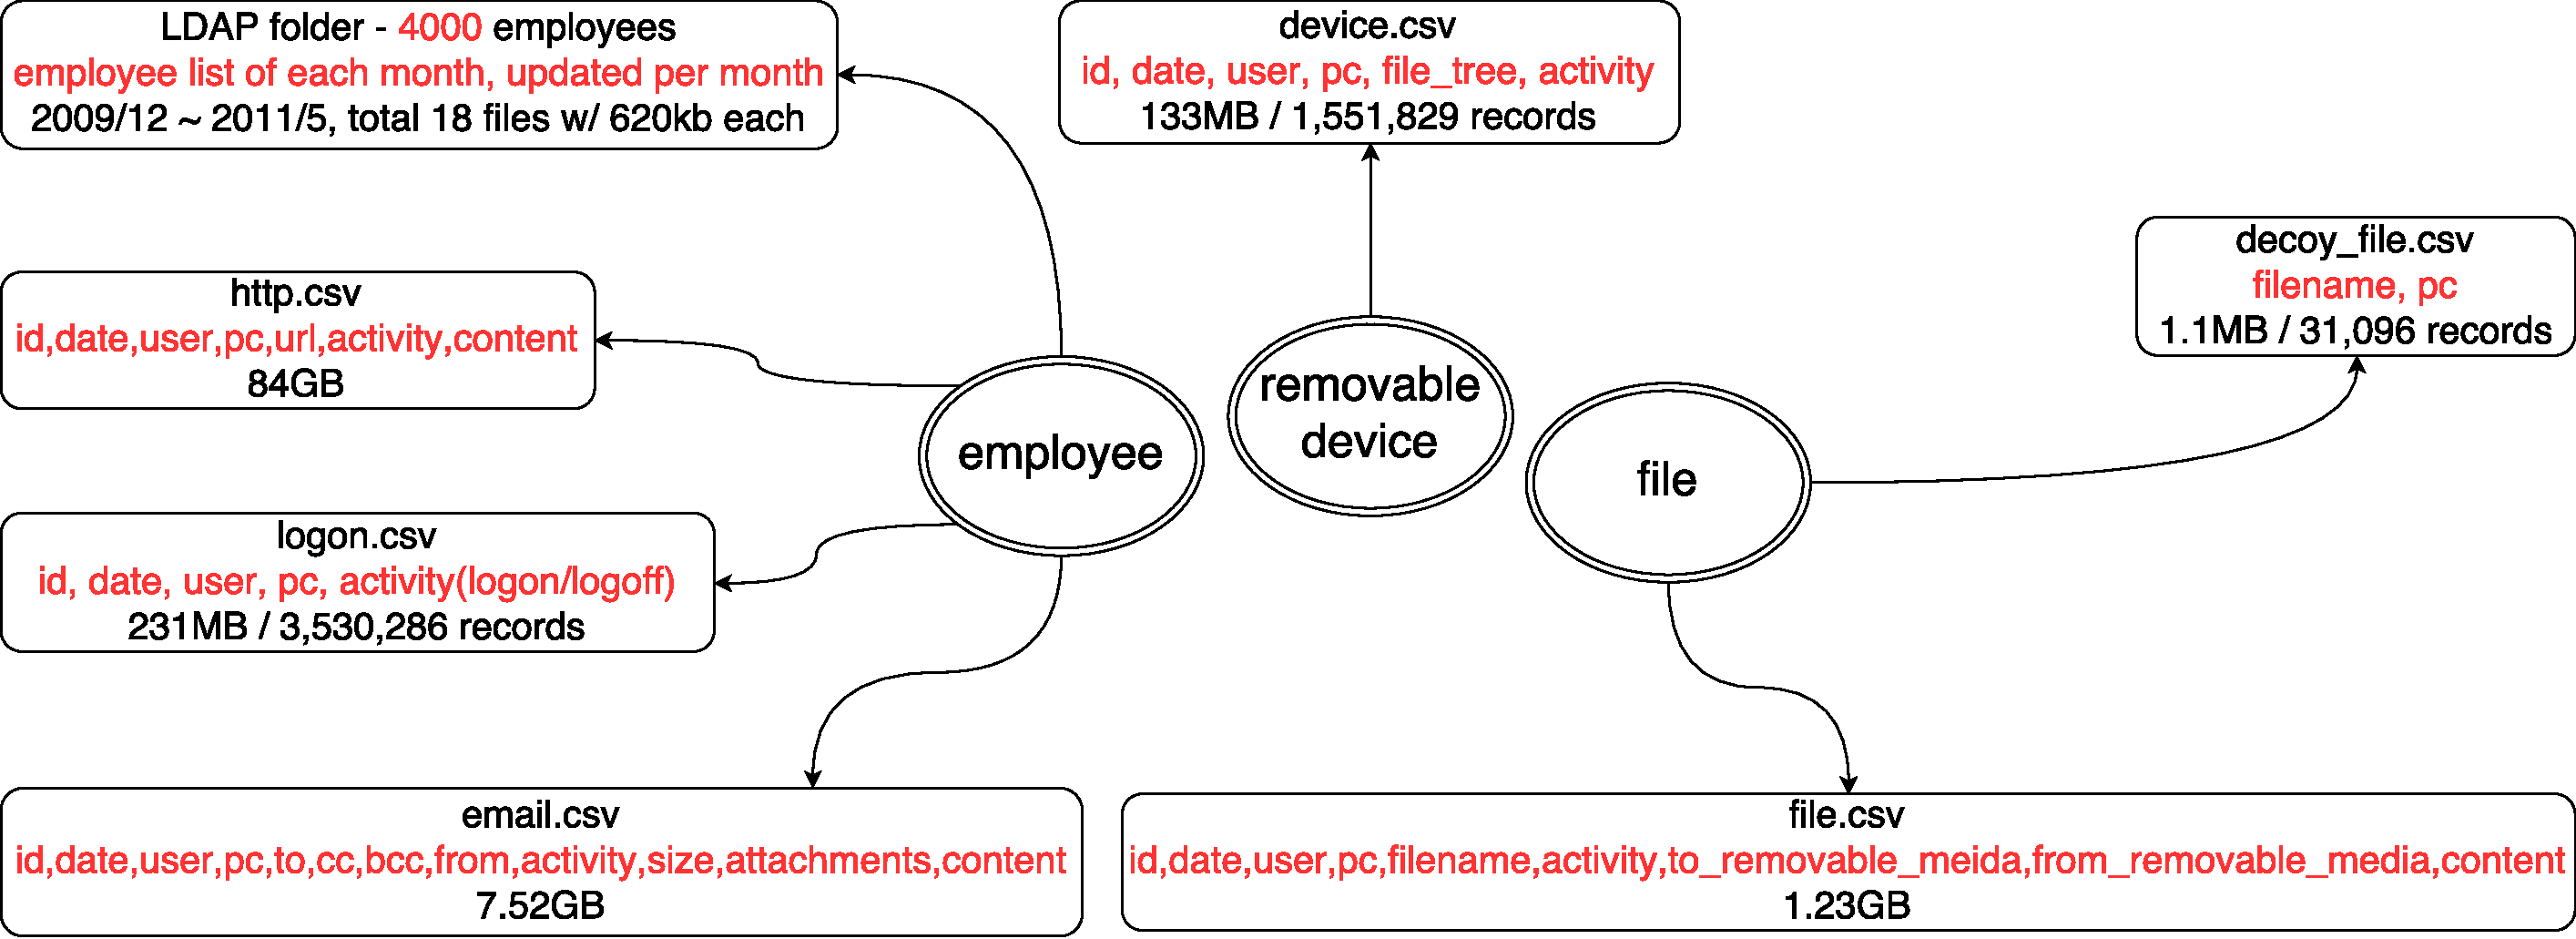
\includegraphics[width=5in]{img/5-dxd.pdf}
    \caption{\textbf{Synthesized Data for Insider Threat Detection}}
    \label{fig:dxd}
\end{figure}

This figure indicates that the dataset is big in size and rich in content. 
It contains 3 categories, the employee data, the removable device data, and the file data. 
An employee can be seen as a sensor that constantly streams action data over a time line, such as HTTP actions including browsing, downloading, and uploading; 
log-on, log-off actions on the organization computers; as well as email actions.
The removable device data includes the actions of using a certain removable device (such as a flash drive) to transfer data.
The file data includes the employee actions performed on the file, such as the contents of the file copied.
There is also some background information provided in the dataset, such as LDAP data in the employee category and the decoy-file data in the file category. 
The LDAP data contains the full list of employees, with their roles, office location and working relationships. 
This list updates weekly. 
The decoy-file data contains the files that are deliberately placed in the employees' working computers, and works like a bait. 
Each dataset has its own data-schema, and is encoded in the comma separated value format.

This dataset provides 4000 users' actions data, in which 5 users are malicious insiders. 
From the given brief scenarios descriptions in the data set, 4 out of 5 malicious insiders are data exfiltration insiders. 
For more details about the dataset, please refer to the \cite{glasser2013bridging} and the website: https://www.cert.org/insider$-$threat/tools/.
%
\subsection{Ontology}
CMU CERT has developed an insider threat indicator ontology \cite{costa2014ontology}.
This ontology primarily contains the concepts and relationships that are extracted from their real insider threat use case events database. 
This ontology is leveraged to describe the insider threat scenarios instead of natural language for the purpose of providing structured data for machines to process. 
The ontology doesn't contain any specific concepts to model data exfiltration. 
It is either inconsistent: 
the concept \textbf{TradeSecretInformation} is classified to be both \textbf{Asset} and \textbf{Information}, which are disjoint classes.
In order to extend the CERT ontology, the inconsistency problem needs to be addressed\footnote{I have contacted CMU CERT and provided this feedback to them.}. 
Currently, it is solved by removing the disjointness.
The ontology of this use case is modeled as the figures below. 

\begin{figure}[!htbp]
	\centering
    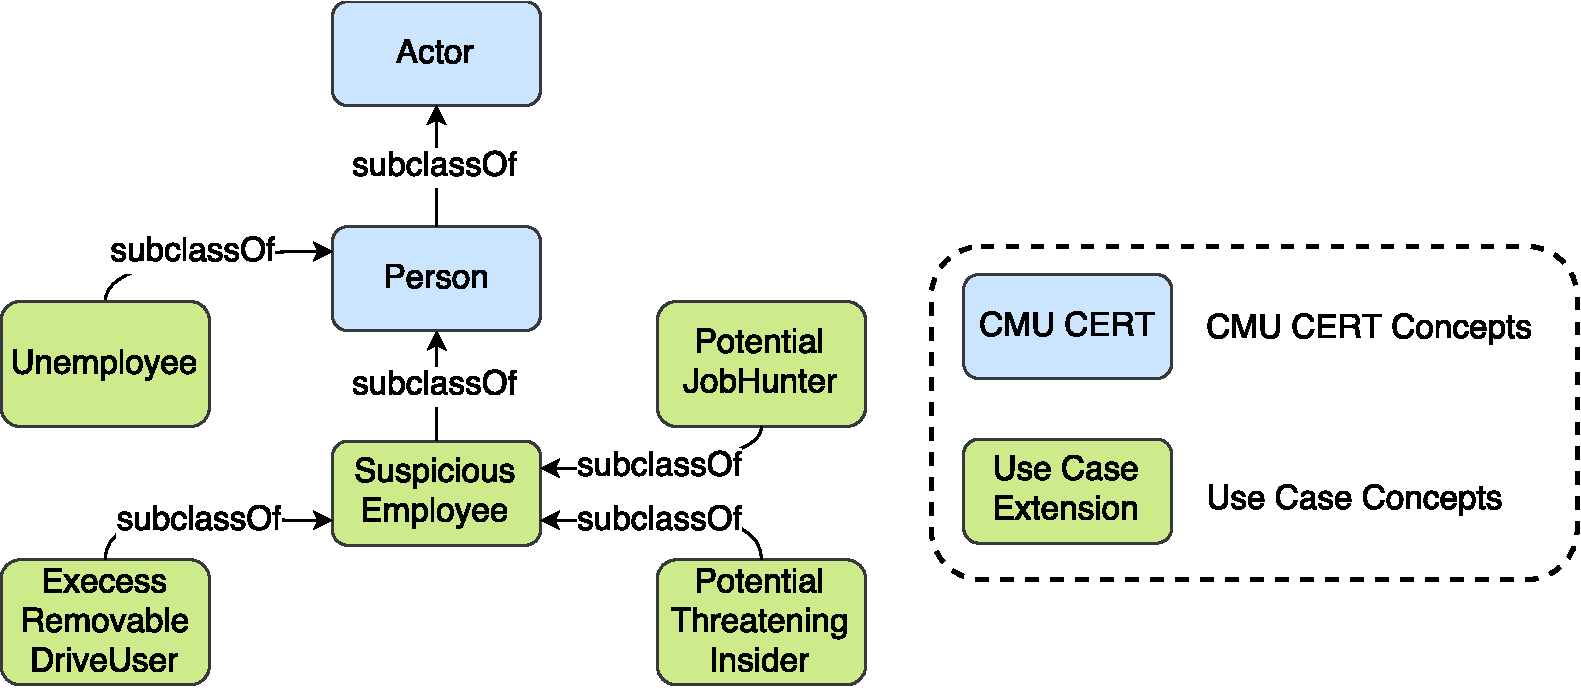
\includegraphics[width=5in]{img/5-dxoactor.pdf}
    \caption{\textbf{Data Exfiltration Background Ontology: Actor}}
    \label{fig:actor}
\end{figure}

Figure \ref{fig:actor} extends the concept \textbf{Actor} by introducing 5 subclasses. 
\textbf{Unemployee} and \textbf{SuspiciousEmployee} are both subclasses of \textbf{Person}.
\textbf{Unemployee} describes previous employees who left the job (either resignation, or laid-off). 
\textbf{SuspiciousEmployee} has three subclasses:
\textbf{ExcessiveRemovableDriveUser} class describes a user who excessively uses the removable disk, compared to his/her normal daily removable disk usage. 
\textbf{PotentialJobHunter} class describes an employee who browsed some job hunting website. 
It's not necessary for an employee to be a jobhunter if he browses job-related website, but the system should be able to record it, then fire an alarm if further suspicious events are detected. 
This class is defined as (\textit{browseWebsite some} \textbf{JobHuntingWebsite}). 
\textbf{PotentialThreateningInsider} class describes a potential threatening insider.
The reason not to name it as something like ``a threatening insider'' is because humans are needed to make the final decision. 
Any users classified into this class will become the forensic target, and is what this use case is looking for. 
This class is defined as (\textit{isInvolvedIn some} \textbf{DataExfiltrationEvent}). 

\begin{figure}[!htbp]
	\centering
    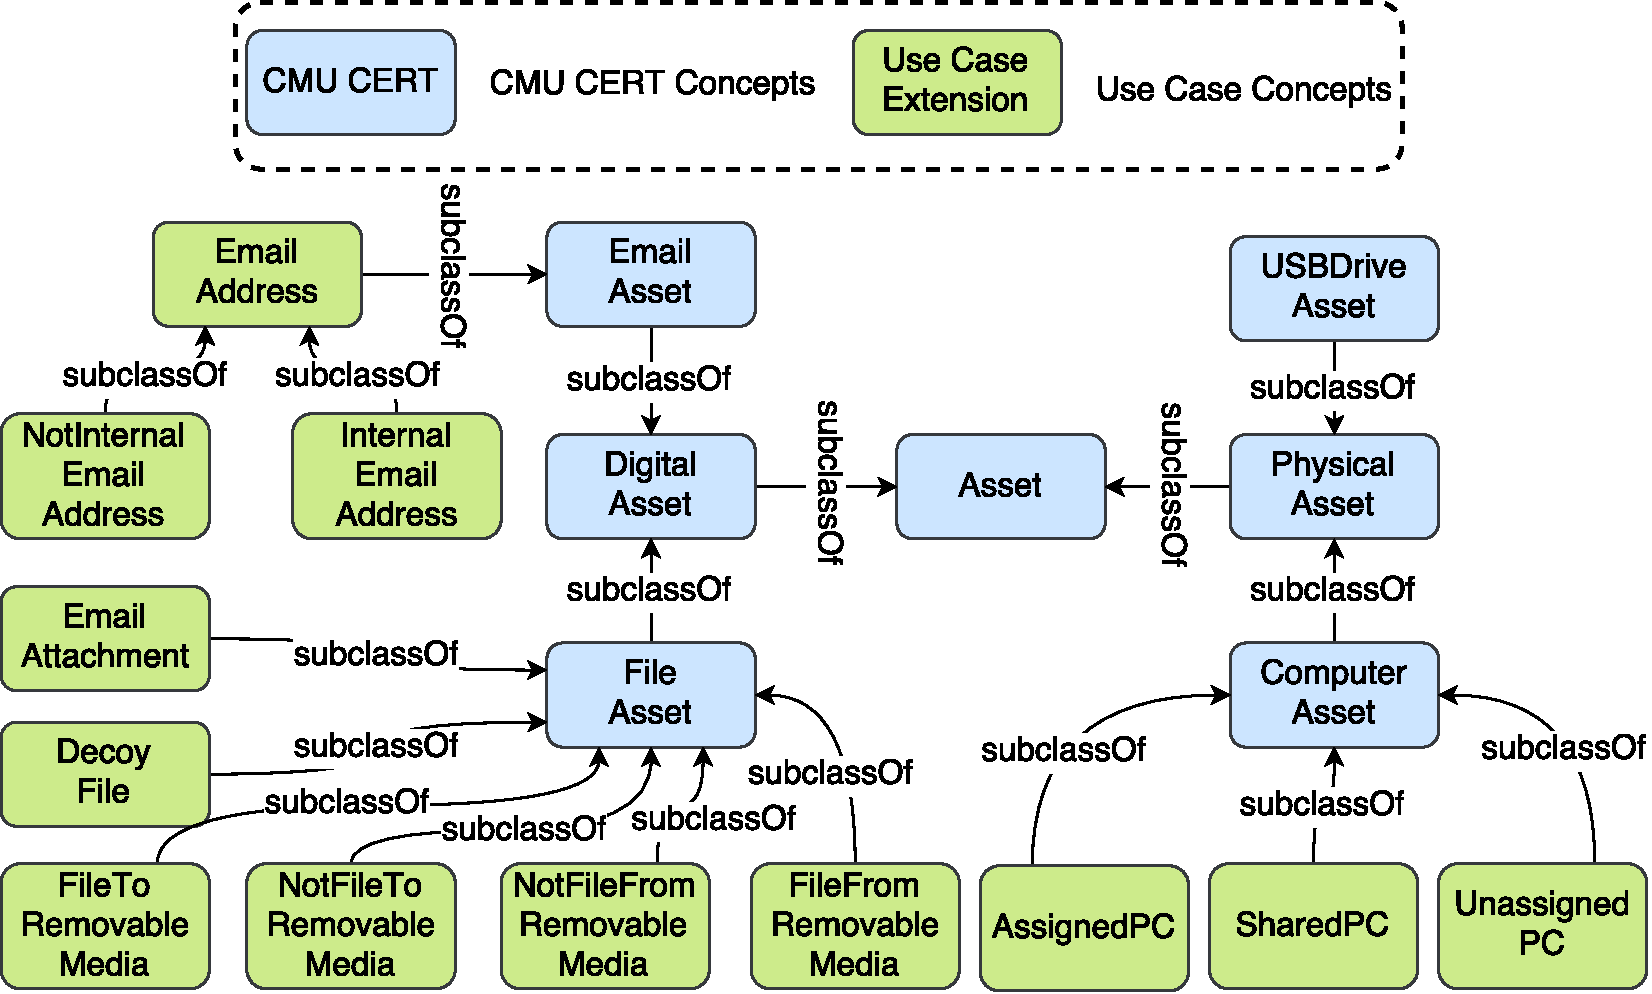
\includegraphics[width=5in]{img/5-dxoasset.pdf}
    \caption{\textbf{Data Exfiltration Background Ontology: Asset}}
    \label{fig:asset}
\end{figure}

Figure \ref{fig:asset} shows the extended models for \textbf{Asset} class.
The focus of using this class is to model the email addresses, files and computers. 
For example, it is important to classify the emails sent to an internal address or an external address. 
It is also crucial to know what kind of file is attached to the email, or copied to/from the flash drive. 
Being able to record which employee uses which computer is also necessary since malicious insiders can possibly get on other employees' computers to steal data. 

\begin{figure}[!htbp]
	\centering
    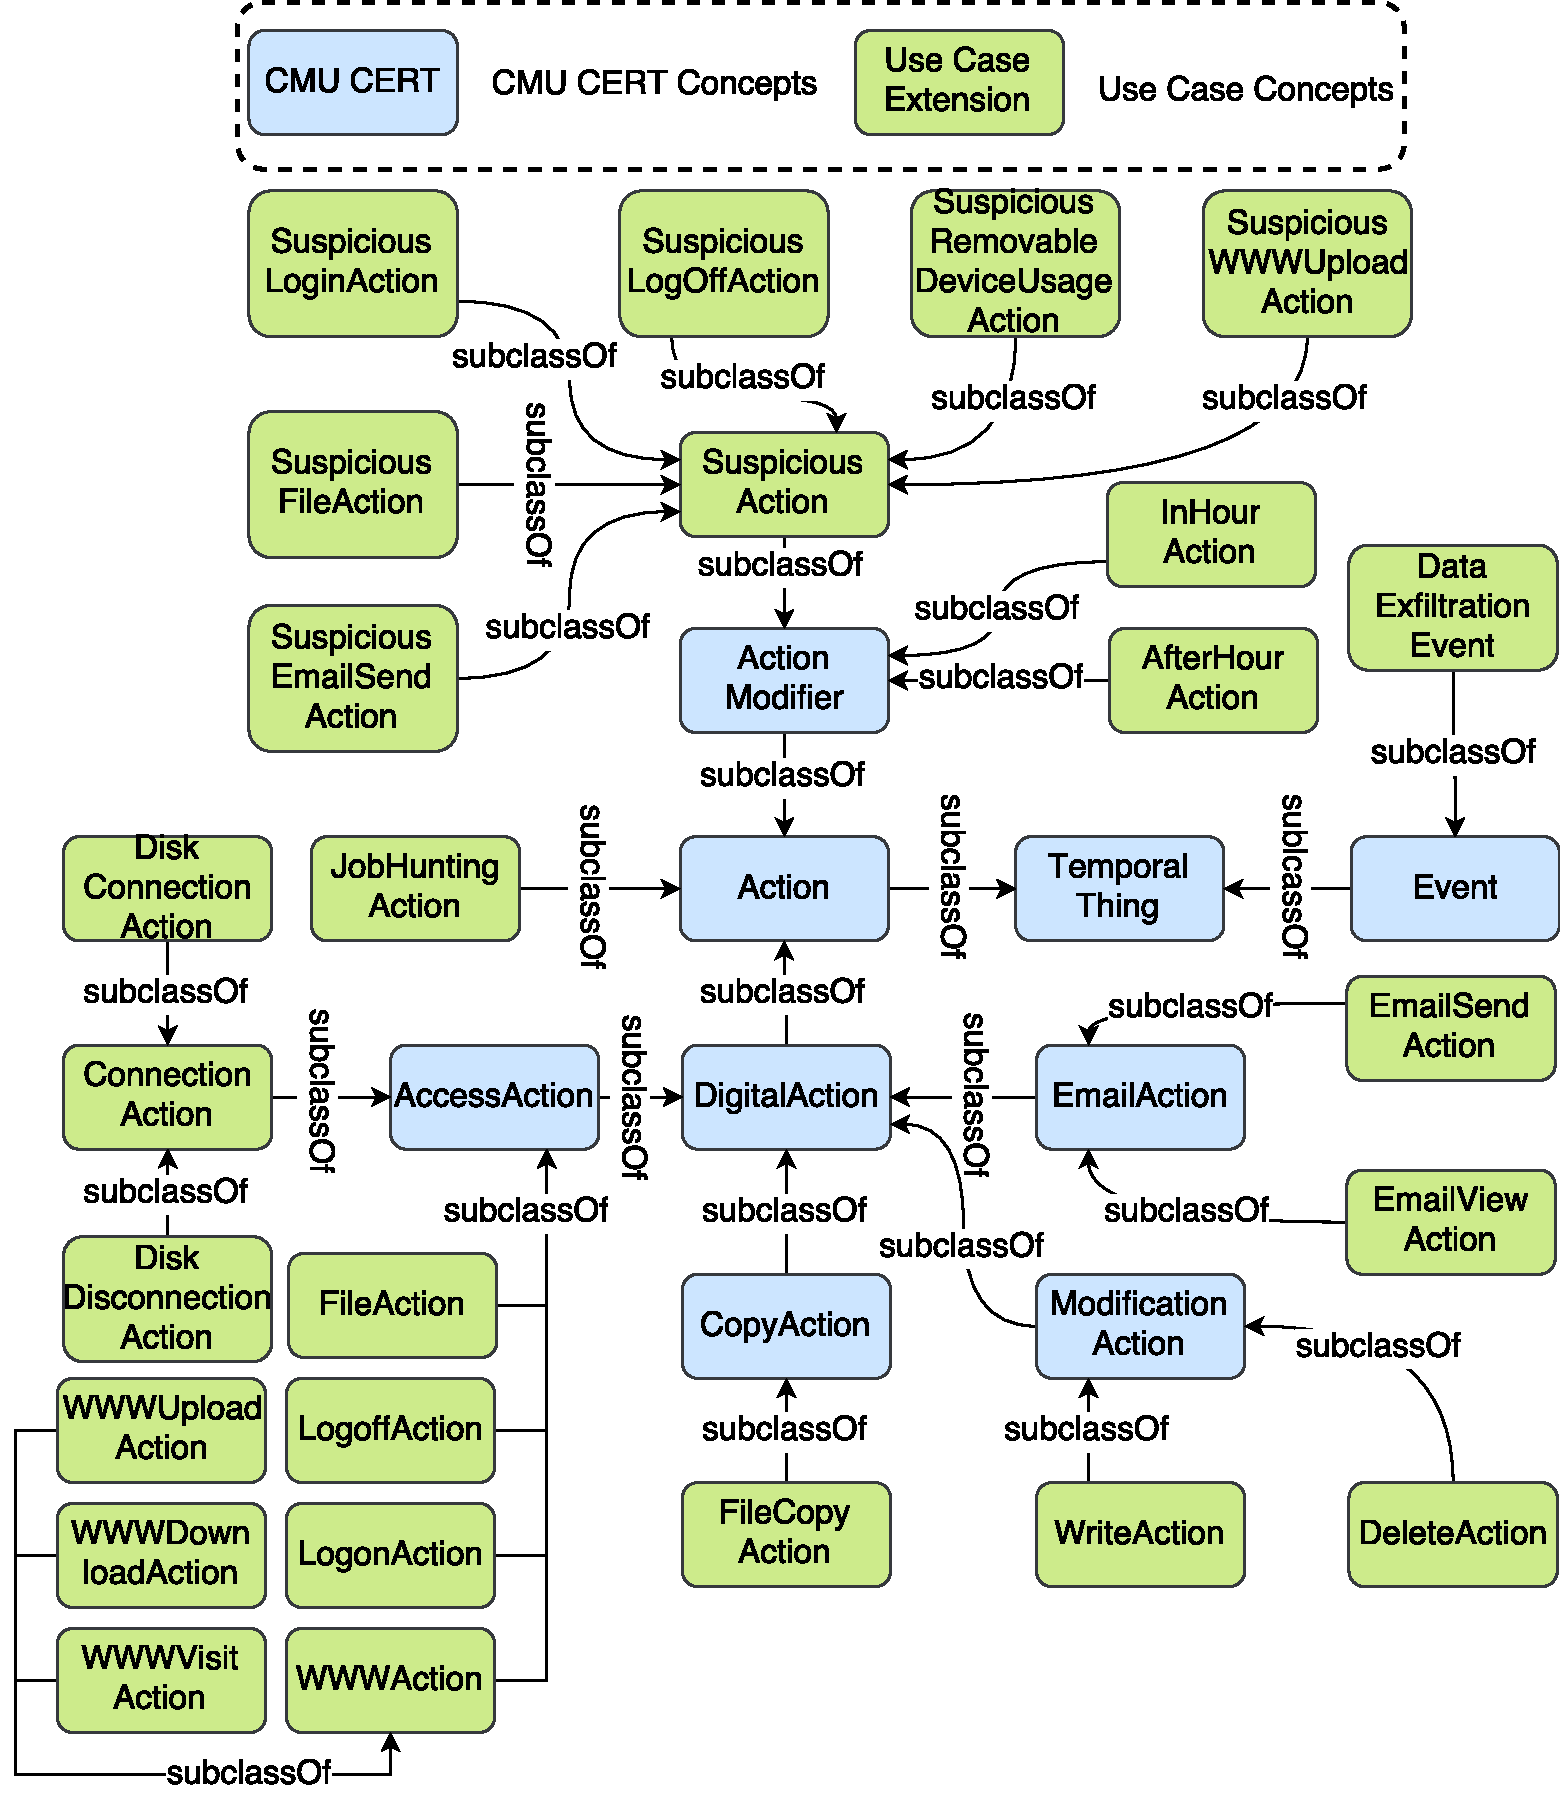
\includegraphics[width=5in]{img/5-dxott.pdf}
    \caption{\textbf{Data Exfiltration Background Ontology: Temporal Thing}}
    \label{fig:tt}
\end{figure}

In the CMU ontology, \textbf{TemporalThing} is the superclass of \textbf{Action} and 
\textbf{Event}, as both of them are time sensitive. 
\textbf{ActionModifier} describes the kinds of the action. 
For example, \textbf{AfterHourAction} describes an action that happens after hour. 
The \textbf{SuspiciousAction} is defined as (\textbf{JobHuntingAction} \textit{or} \textbf{SuspiciousEmailSendAction} \textit{or} \textbf{SuspiciousFileAction} \textit{or} \textbf{SuspiciousLoginAction} \textit{or} \textbf{SuspiciousRemovableDeviceUsageAction} \textit{or} \textbf{SuspiciousWWWUploadAction}). 
This class classifies the defined suspicious actions. 
The reason to include the \textbf{JobHuntingAction} is because a potential job hunter should be taken care of. 
All of the subclasses of \textbf{SuspiciousAction} are defined, which provides the known data exfiltration patterns. 

\textbf{SuspiciousEmailSendAction} is defined as (\textbf{EmailSendAction} \textit{and} ((\textit{bcc some} \textbf{NotInternalEmailAddress}) \textit{or} (\textit{cc some} \textbf{NotInternalEmailAddress}) \textit{or} (\textit{from some} \textbf{NotInternalEmailAddress}) \textit{or} (\textit{to some} \textbf{NotInternalEmailAddress}))) \textit{or} (\textit{hasEmailAttachment some} \textbf{DecoyFile}).
It takes care of those emails sent to external email addresses. 

\textbf{SuspiciousFileAction} is defined as (\textbf{AfterHourAction} \textit{and} ( \textbf{FileCopyAction} \textit{or} \textbf{FileDeleteAction} \textit{or} \textbf{FileOpenAction})) \textit{or} (\textbf{FileCopyAction} \textit{and} (\textit{hasFile some} \textbf{DecoyFile})) \textit{or} (((\textit{isPerformedOnPC some} \textbf{UnassignedPC}) \textit{and} \textbf{FileCopyAction} \textit{or} \textbf{FileDeleteAction} \textit{or}  \textbf{FileOpenAction})) \textit{or} (\textit{startsNoEarlierThanEndingOf some} \textbf{SuspiciousRemovableDeviceUsageAction}). 
Basically, a suspicious file action is an action that either is performed after hour by deleting, copying or opening a decoy file, or using a removable drive to delete, copy, or open files on an unassigned PC. 

\textbf{SuspiciousLoginAction} is defined as (\textbf{AfterHourAction} \textit{and} \textbf{LogonAction}) \textit{or} (\textbf{LogonAction} \textit{and} (\textit{isPerformedOnPC some} \textbf{UnassignedPC})).
This means that any action that is performed after hours or on an unassigned PC will be classified as a suspicious login action. 
Similarly, \textbf{SuspiciousLogoffAction} is defined as (\textbf{AfterHourAction} \textit{and} \textbf{LogoffAction}) \textit{or} (\textbf{LogoffAction} \textit{and} (\textit{isPerformedOnPC some} \textbf{UnassignedPC})).

\textbf{SuspiciousRemovableDeviceUsageAction} is defined as ( \textbf{AfterHourAction} \textit{and} (\textbf{DiskConnectionAction} \textit{or} \textbf{DiskDisconnectionAction})) \textit{or} ((\textbf{DiskC\\onnectionAction} \textit{or} \textbf{DiskDisconnectionAction}) \textit{and} (\textit{isPerformedOnUnassign\\edPC some} \textbf{UnassignedPC})) \textit{or} (\textit{hasActor some} \textbf{ExcessiveRemovableDriveUs\\er}).
This class will classify the actions that are performed either after hours with a disk connection action, or from an excessive removable driver user. 

\textbf{SuspiciousWWWUploadAction} is defined as (\textbf{AfterHourAction} \textit{and} \textbf{W\\WWUploadAction}) \textit{or} (\textbf{WWWUploadAction} \textit{and} (\textit{hasWebsite some} (\textbf{Cloud\\StorageWebsite} \textit{or} \textbf{HacktivistWebsite}))) \textit{or} ((\textbf{WWWDownloadAction} \textit{or} \textbf{WWWUploadAction} \textit{or} \textbf{WWWVisitAction}) \textit{and} (\textit{isPerformedOnUnassigned\\PC some} \textbf{Unassigned-PC})).
It describes a kind of malicious action that a user uploads files to cloud storage or hactivist website after-hour or from an unsigned PC.

\textbf{DataExfiltrationEvent} class is the subclass of \textbf{Event}. 
It describes the data exfiltration event, and is defined as ((((\textit{hasAction min 10} \textbf{SuspiciousEmailSendAction}) \textit{and} (\textit{hasAction max 10000} \textbf{SuspiciousEmailSendAction})) \textit{or} (\textit{hasAction max 10000} \textbf{SuspiciousWWWUploadAction})) \textit{and} (\textit{hasAction min 5} \textbf{SuspiciousWWWUploadAction})) \textit{or} ((\textit{hasAction min 3} \textbf{SuspiciousFileAction}) \textit{and} (\textit{hasAction max 10000} \textbf{SuspiciousFileAction})).
In its definition, cardinality is used to quantify a threshold to determine a data exfiltration event.

Last but not the least, the ontology has a \textbf{Website} class that models different websites. 
It has four subclasses, \textbf{CloudStorageWebsite} that describes sites like dropbox.com; 
\textbf{HacktivistWebsite} that describes sites like wikileaks.org;
\textbf{JobHuntingWebsite} that describes sites like indeed.com;
and \textbf{NeutralWebsite} that describes sites other than the above three. 

\subsection{Data Annotation}
Data is pre-processed before annotated by the data exfiltration background ontology. 
All employees' routine hours are calculated based on their first two week working hours. 
This routine hours will be used as a basis of judging the after hour actions. 
Also, employees' routine log-on/log-off time, and daily removable disk usage situations are extracted for reference. 
In the LDAP folder of the synthesized dataset, a employee list is provided for every month.
This list is updated monthly, thus employees who are not in current month LDAP list will be annotated as an instance of \textbf{Unemployee}.

Logon.csv file follows the schema of (id, date, user, pc, activity), where ``id'' is the unique action id, ``date'' is a xsd:dateTime timestamp indicating the generation timestamp of the action, ``user'' is the employee id, ``pc'' is where the action is performed, ``activity'' is a string of either logon or logoff. 
Thus, the data in Logon.csv file can be annotated in RDF stream as follows: \\
(1) :$<$user$>$-event :hasAction :$<$activity$>$\_$<$id$>$, $<$date$>$. \\
(2) :$<$activity$>$\_$<$id$>$ rdf:type :Action, $<$date$>$. \\
(3) if $<$date$>$ is not in normal working hours of $<$user$>$, \\
:$<$activity$>$\_$<$id$>$ rdf:type :AfterHourAction, $<$date$>$; \\ 
else, :$<$activity$>$\_$<$id$>$ rdf:type :InHourAction, $<$date$>$. \\
(4) :$<$activity$>$\_$<$id$>$ :hasActor :$<$user$>$, $<$date$>$.  \\
(5) :$<$activity$>$\_$<$id$>$ :isPerformedOnPC :$<$pc$>$, $<$date$>$. 

Device.csv file has the schema of (id, date, user, pc, file\_tree, activity), where ``id, date, user, pc'' are the same as Logon.csv.
``file\_tree'' is the directory content of the removable drive.
``activity'' describes the action taken by the user. 
The data is annotated as follows: \\
(1) :$<$user$>$-event :hasAction :device\_$<$activity$>$\_$<$id$>$, $<$date$>$. \\
(2) if current employee's daily removable device usage count is bigger than his/her routine usage, then annotate \\
:$<$user$>$ rdf:type :ExcessiveRemovableDriveUser, $<$date$>$. \\
(3) :device\_$<$activity$>$\_$<$id$>$ rdf:type :Action, $<$date$>$. \\
(4) if $<$date$>$ is not in the normal working hours of $<$user$>$, \\
:device\_$<$activity$>$\_$<$id$>$ rdf:type :AfterHourAction, $<$date$>$; \\
else, :device\_$<$activity$>$\_$<$id$>$ rdf:type :InHourAction, $<$date$>$. \\
(5) :device\_$<$activity$>$\_$<$id$>$ :hasActor :$<$user$>$, $<$date$>$. \\
(6) :device\_$<$activity$>$\_$<$id$>$ :isPerformedOnPC :$<$pc$>$, $<$date$>$. \\
(7) if the activity is ``connect'', \\
:device\_$<$activity$>$\_$<$id$>$ :isPerformedWithRemovableDisk \\
:device\_$<$activity$>$\_$<$id$>$\_disk, $<$date$>$. 

Email.csv file encodes data with the schema of (id, date, user, pc, to, cc, bcc, from, activity, size, attachments, content), where ``id, date, user, pc'' are the same as above. 
``to, cc, bcc, from'' respectively indicates the sender's and receivers' email addresses, ``activity'' is either send or view, ``size'' is the attachment's size in bytes, ``attachments'' refer to the attached files in the email, ``content'' indicates the contents in the email. 
The data is annotated as follows: \\
(1) $<$user$>$-event :hasAction :email\_$<$activity$>$\_$<$id$>$, $<$date$>$. \\
(2) :email\_$<$activity$>$\_$<$id$>$ rdf:type :EmailAction, $<$date$>$. \\
(3) if $<$date$>$ is not in the normal working hours, \\
:email\_$<$activity$>$\_$<$id$>$ rdf:type :AfterHourAction, $<$date$>$; \\
else, :email\_$<$activity$>$\_$<$id$>$ rdf:type :InHourAction, $<$date$>$. \\ 
(4) :email\_$<$activity$>$\_$<$id$>$ :hasActor $<$user$>$, $<$date$>$. \\
(5) :email\_$<$activity$>$\_$<$id$>$ :isPerformedOnPC $<$pc$>$, $<$date$>$.\\ 
(6) :email\_$<$activity$>$\_$<$id$>$ :to :$<$to$>$, $<$date$>$,\\
(7) :email\_$<$activity$>$\_$<$id$>$ :cc :$<$cc$>$, $<$date$>$. \\
(8) :email\_$<$activity$>$\_$<$id$>$ :bcc :$<$bcc$>$, $<$date$<$. \\
(9) :email\_$<$activity$>$\_$<$id$>$ :from :$<$from$>$, $<$date$>$. \\
(10) if the email address ($<$email-address$>$ includes $<$to$>$, $<$cc$>$, $<$bcc$>$, and $<$from$>$) is the organization address,\\
:$<$email-address$>$ rdf:type :InternalEmailAddress;\\
else, :$<$email-address$>$ rdf:type :ExternalEmailAddress.\\ 
(11) :email\_$<$activity$>$\_$<$id$>$ :hasEmailAttachment :$<$attachments$>$, $<$date$>$. \\
(12) :$<$attachments$>$ :hasSize :$<$size$>$, $<$date$>$.\\
(13) :email\_$<$activity$>$\_$<$id$>$ :hasContent :$<$content$>$, $<$date$>$. 

File.csv file contains the data schema of (id, date, user, pc, filename, activity, to\_removable\_media, from\_removable\_media, content), where ``id, date, user, pc'' are the same as the above.
``filename'' describes the name of the file, ``activity'' denotes the action performed on the file, ``to\_removable\_media'' denotes if the file is performed to the removable media, ``from\_removable\_media'' is the opposite, ``content'' describes the file content. 
The data is annotated as follows: \\
(1) :$<$user$>$-event :hasAction :file\_$<$activity$>$\_$<$id$>$, $<$date$>$. \\
(2) :file\_$<$activity$>$\_$<$id$>$ rdf:type :FileAction, $<$date$>$. \\
(3) if $<$date$>$ is not within the normal working hours, \\
:file\_$<$activity$>$\_$<$id$>$ rdf:type :AfterHourAction, $<$date$>$;\\
else, :file\_$<$activity$>$\_$<$id$>$ rdf:type :InHourAction, $<$date$>$.\\ 
(4) :file\_$<$activity$>$\_$<$id$>$ :hasActor :$<$user$>$, $<$date$>$. \\
(5) :file\_$<$activity$>$\_$<$id$>$ :isPerformedOnPC :$<$pc$>$, $<$date$>$. \\
(6) :file\_$<$activity$>$\_$<$id$>$ :hasFile :$<$filename$>$, $<$date$>$.\\
(7) if ``to\_removable\_media" is true, \\
:$<$filename$>$ rdf:type :FileToRemovableMedia, $<$date$>$;\\
else, $<$filename$>$ rdf:type NotFileToRemovableMedia, $<$date$>$.\\ 
(8) if ``from\_removable\_media'' is true,\\
:$<$filename$>$ rdf:type :FileFromRemovableMedia, $<$date$>$;\\
else, $<$filename$>$ rdf:type :NotFileFromRemovableMedia, $<$date$>$. 

Decoy.csv has the data schema of ``filename, pc'', where ``filename'' is the name of the decoy file, ``pc'' is where the file is located.
Decoy.csv file is used as the background information, thus no timestamps are associated. 
Data is annotated as: \\
(1) :$<$filename$>$ rdf:type :DecoyFile. \\
(2) :$<$filename$>$ :isIn $<$pc$>$. 

LDAP folder contains 18 files, each of which is a list of employees during that month.
They record from 2009/12 to 2011/05.
The employee list is updated monthly.
These files are used as the background information. 
Each file is with a data schema of (employee\_name, user\_id, email, role, projects, business\_unit, functional\_unit, department, team, supervisor).
Thus the data is annotated as: \\
(1) :$<$user\_id$>$ :hasName :$<$employee\_name$>$. \\
(2) :$<$user\_id$>$ :hasEmailAddress :$<$email$>$. \\
(3) :$<$user\_id$>$ :hasRole :$<$role$>$. \\
(4) :$<$user\_id$>$ :hasProjects :$<$projects$>$. \\
(5) :$<$user\_id$>$ :hasBusinessUnit :$<$business\_unit$>$. \\
(6) :$<$user\_id$>$ :hasFunctionalUnit :$<$functional\_unit$>$. \\
(7) :$<$user\_id$>$ :hasDepartment :$<$department$>$. \\
(8) :$<$user\_id$>$ :hasTeam :$<$team$>$. \\
(9) :$<$user\_id$>$ :hasSupervisor :$<$supervisor$>$.

Http.csv file has the schema of ``id, date, user, pc, url, activity, content'', where ``id, date, user, pc'' are the same as the above. 
``url'' is the link that the user visits, ``activity'' is either view, upload, and download, ``content'' is the content of the web-page browsed. 
The data is annotated as follows:\\
(1) :$<$user$>$-event :hasAction :http\_$<$activity$>$\_$<$id$>$, $<$date$>$.\\
(2) :http\_$<$activity$>$\_$<$id$>$ rdf:type :Action, $<$date$>$.\\
(3) if $<$date$>$ is within the routine hours of the user, \\
:http\_$<$activity$>$\_$<$id$>$ rdf:type :InHourAction, $<$date$>$;\\
else, :http\_$<$activity$>$\_$<$id$>$ rdf:type :AfterHourAction, $<$date$>$.\\
(4) :http\_$<$activity$>$\_$<$id$>$ :hasActor :$<$user$>$, $<$date$>$.\\
(5) :http\_$<$activity$>$\_$<$id$>$ :isPerformedOnPC :$<$pc$>$, $<$date$>$.\\
(6) :http\_$<$activity$>$\_$<$id$>$ :hasURL :$<$url$>$, $<$date$>$.\\
(7) URLs are annotated with \textbf{Website} class: \\
:$<$url$>$ :whoseDomainNameIsA :cloudstoragewebsite \\
:$<$url$>$ :whoseDomainNameIsA :hacktivistwebsite \\
:$<$url$>$ :whoseDomainNameIsA :jobhuntingwebsite \\
:$<$url$>$ :whoseDomainNameIsA :neutralwebsite.
%
\subsection{System Implementation}
The data exfiltration detection system is implemented on the basis of the sequential stream reasoning architecture. 
A lower-bounded landmark logical window is deployed in the system. 
The advantage of the landmark window is reflected incisively and vividly in this use case. 
For data exfiltration detection, the malicious insiders can do harm to the organization in any arbitrary time period, which makes determining the size for the conventional logical sliding window very challenging: a small size probably will not provide good precision, but a big size will result in more data that hinders the system performance. 
A landmark window, on the other hand, can retain the useful data when evicting other data, and can work with various window management strategies. 

The query is to look for suspicious actions, which is shown in Listing 5.5. 
This query involves the background data such as LDAP, the streaming data annotated by the background ontology as well as the background ontology itself.
This query requires DL reasoning. 

\begin{lstlisting}[caption={\textbf{Suspicious Action Query}},basicstyle=\small]
PREFIX de:<http://tw.rpi.edu/ontology/DataExfiltration/>
SELECT DISTINCT ?action 
WHERE { 
    ?action a de:SuspiciousAction.
}
\end{lstlisting}

Employees who performed the detected suspicious actions will be recorded, together with the actions he/she performs. 
All of the records will be printed to the screen, written to the event log, and make it easier for humans to make a final judgment. 
However, detecting suspicious actions is not the ultimate goal of this use case.
In the background ontology, the data exfiltration event is defined with cardinalities.
If an employee performs suspicious actions several times, then this employee is a potential malicious insider, and should be paid special attention to. 
Thus, another query in Listing 5.6 examines the employees' performed suspicious actions and checks if he/she is a potential malicious insider. 
This query is parameterized, where $<$user$>$ will be filled during the run time. 
If this query returns true, then the user will be reported. 
The query also requires DL reasoning. 

\begin{lstlisting}[ caption={\textbf{Potential Malicious Insider Query}},basicstyle=\small]
PREFIX de:<http://tw.rpi.edu/ontology/DataExfiltration/>
ASK WHERE { 
    de:<user> a de:PotentialThreateningInsider.
}
\end{lstlisting}

This use case has chosen provenance and trustworthiness from semantic importance to form two window management strategies, FIFO and QR-T. 
FIFO is first in first out, its priority vector is [$\tau_{a}$]; 
while QR-T is query relevance trustworthiness, its priority vector is [$qrf, t^{tm}_{s}$]
The reason to choose query relevance is because of the large amount of the streaming data. 
There is really a need to identify, and filter out the unnecessary data to improve system response. 
Thus, a query relevance ontology is provided. 
In the previous section, it is mentioned that this query relevance ontology is query-informed.
However, for this use case, no dedicated query relevance ontology is provided, as the background domain ontology has already provided enough information to filter out the data. 
In this use case, the background domain ontology can be used as a query relevance ontology. 
For example, the query in Listing 5.5 really looks for the suspicious actions. 
As the action data keeps streaming into the system, each action data item will be examined by the query engine, and if that action data item is not classified as a suspicious action, it can be immediately dropped without having to enter into the window.
Only those suspicious action instances will be entered into the window. 
One important thing to note is that, the reason this use case implementation can realize query relevance filtering with a background ontology is very use case specific, and should not be seen as a general solution. 
This use case can do this because the background ontology has already provide enough information, as well as the system working mechanism that each action data item will be examined before entering into the window. 

A simple trust mode has been developed because the existing models are very heterogeneous, and not usually applicable for the scenario of this use case. 
The trust model works in this way: 
initially, each employee has a trust score of $t_{s_i}$. 
As the system runs, if an employee A performed a suspicious action, his/her trust score will reduce 1. 
There is a threshold Y, such that $0 < Y < t_{s_i}$. 
If A's $t^{A}_{s_i}$ is smaller than Y, then  employee A becomes untrusted, thus all of his/her actions will be recorded and sent to the administrators to analyze. 
The QR-T strategy firstly filters out the unnecessary action data, then ranks the action data according to their actors' trust scores. 
%
\subsection{Evaluation}
The window has been set to detect the period of 1 day, 1 week and 1 month for any suspicious actions and malicious users. 
Two strategies are deployed, and evaluated via recording the precision, recall, and the running time. 

\begin{table}[!htbp]
	\centering
    \caption{\textbf{Strategy Performance}}
    \label{tab:sp}
    \begin{tabular}{|c||c|c|} \hline
    	& precision & recall \\ \hhline{|=#=|=|}
        FIFO (1D) & 0.18 & 0.93 \\ \hline
        QR-T (1D) & 0.18 & 0.97 \\ \hline
        FIFO (1W) & 0.26 & 0.87 \\ \hline
        QR-T (1W) & 0.26 & 0.95 \\ \hline
        FIFO (1M) & 0.26 & 0.87 \\ \hline
        QR-T (1M) & 0.26 & 0.95 \\ \hline
    \end{tabular}
\end{table}

Table \ref{tab:sp} shows the system precision and recall. 
The precision of FIFO and QR-T are equal for the same detection time period, and slightly increases as the time-period becomes bigger. 
QR-T's recall is always better than that of FIFO for the same detection time period. 
The precision, undoubtedly, is very low. 
There are reasons for that. 
Insider threat is by no means a simple problem that can be solved with only stream reasoning technologies, it should at least include natural language processing, machine learning and possibily some other technologies. 
The known pattern on data exfiltration is not very discriminative.
That a person who uses a removable disk to copy some file and then upload it into dropbox could be either malicious or innocent.
Thus the background ontology cannot do a good job in classifying data exfiltration actions.

\begin{table}[!htbp]
	\centering
    \caption{\textbf{Strategy Running Time}}
    \label{tab:srt}
    \begin{tabular}{|c||c|c|} \hline
	    & FIFO & QR-T \\ \hhline{|=#=|=|}
    	$T_{total}$ & 49.94 (ms) & 29.63 (ms) \\ \hline    
    \end{tabular}	
\end{table}

However, this use case implementation shows a positive example in Table \ref{tab:srt}, where clearly QR-T runs faster than FIFO. 
This is because FIFO strategy has more data in the window than QR-T, which slows down the running performance.
The results have shown that semantic importance enabled window management strategy can improve the system response time. 
%
\section{Discussion}
This section covers the two use case implementations using both semantic importance and sequential stream reasoning architecture.
From the result tables, a significant difference can be seen in the system outputs from different window management strategies enabled by different semantic importance aspects. 
The two use cases, albeit are from two different domains, share similar characters. 
The streaming data is big for both cases. 
The offside use case data updates frequently, while the data exfiltration data is massive due to frequent actions from many employees. 
Also, it requires complex DL reasoning in both cases. 
Streaming data alone, although provides the basic semantics from the ontology annotation, is not able to provide the desired results. 
From the results, we can see that semantic importance is able to improve the system precision, memory consumption, and response time.

Event calculus \cite{khandelwal2013furthering} is for reasoning about changes, which is a different way to implement soccer offside use case. 
However, in order to make event calculus useful, the stream should contain events. 
The original streaming data is only about primitive positional data, there should be some sort of “event detector” plugged in the system, so that different events can be detected, 
then followed by some customized event calculus rules for soccer offside, an offense is reasoned. In our implementation, we use the background ontology as both an event detector, as well as a rule base for soccer offside offence. 
Motif detection \cite{chen2015context} is also another potential way to implement the soccer use case. 
``By definition, the time series motifs are those small segments of temporal varying data that preserve similar patterns and keep reoccurring over time.'' \cite{chen2015context}. 
Since soccer offside offence has a pattern and will recur during the game if it happens, motif detection methods can also be used.
I used sampling to reduce the amount of each sensor’s position data streamed into the system with the premise that sampling does not affect the system output. 
The sampling algorithm is called systematic sampling, which basically means randomly pick up the first element, then pick the next element every k elements away afterwards. 
We use this simple sampling algorithm to reduce the data update frequency but is able to maintain a good sampling result for the use case implementation.

However, one should also see that the implementations of both use cases are dependent upon very specific assumptions that are only applicable in specific scenarios.
This limits the generalization of semantic importance. 
The topics of generalizing and benchmarking semantic importance will be covered in the next chapter. 